% ============================================================================ %
%
%           Šablona bakalářské/diplomové práce
%
% Autor:    Ing. Jozef Říha (2006-05-04), od té doby šablonu udržuje
%           Ing. Pavel Tomášek, Ph.D. (tomasek@utb.cz)
%
% Verze:    2021-05-04
%
% Kódování: UTF-8 (kontrolní řetězec: žluťoučký kůň úpěl ďábelšké ódy)
%
% Sazba:    pdflatex prace.tex && pdflatex prace.tex
%           (nutné dvakrát pro korektní vložení citací a jiných referencí),
%           v případě umístění literatury do externího bib souboru je třeba volat
%           pdflatex prace.tex && bibtex prace && pdflatex prace.tex && pdflatex prace.tex
%
% Tip:      Ve správně vysázeném českém textu by na konci řádku neměla zůstant
%           samotná jednopísmenná předložka či spojka. Na takové místo se vkládá
%           nezalomitelná mezera pomocí symbolu ~. Existuje program, který umí
%           zpracovat celý TeX dokument najednou podle českých konvencí:
%           http://petr.olsak.net/ftp/olsak/vlna/
%
% Pozor:    Vzhledem k požadovanému standardu PDF/A nesmí vložené obrázky 
%           obsahovat alfa kanál (průhlednost).
%
% ============================================================================ %


\documentclass[a4paper,12pt]{article}

% Definice vzhledu a nastavení se načítá z následujícího souboru (netřeba editovat)
% ============================================================================ %
% Tento dokument není zpravidla třeba editovat,
% obsahuje nastavení balíčků, vzhledu, stylů.
%
% Kódování: UTF-8 (žluťoučký kůň úpěl ďábelšké ódy)
% ============================================================================ %


% ============================================================================ %
% BALÍČKY

%\usepackage[czech,english]{babel} % volba při kompilaci latexem (vyžaduje texlive-lang), zakomentovano, nastavovanu prikazem \nastavjazyk
\usepackage[T1]{fontenc}% definice vnitřního kódování
\usepackage[utf8x]{inputenc} % slouží pro definici kódování (při problémech zkusit zaměnit utf8x za utf8)
\usepackage{color}		% umožňuje použití barev
\usepackage{graphicx}	% rozšíření práce s grafikou
\usepackage{amsmath}	% balíček pro pokročilejší matematiku
\usepackage{fancyhdr}	% detailnější nastavení záhlaví a zápatí
\usepackage{tocloft}	% umožňuje pohodlné nastavení vzhledu obsahu, seznamu tabulek či obrázků
\usepackage{textcase}	% změna VeLiKoStI PíSmA
\usepackage{ifthen} 	% balíček umožňující skladby if, then -- využijeme při definici nadpisů
\usepackage{setspace}	% balíček umožňující nastavit řádkování na 1, 1.5, 2
\usepackage{ccaption}	% vylepšení práce s popisky obrázků či tabulek
\usepackage{sectsty}	% pro nastavení vzhledu nadpisů
\usepackage[srcstyle=leftnumhang,linenumbersep={\ }]{examplep} % pokročilejší sazba programového kódu
\usepackage{url}		% balíček pro vysázení internetové adresy stylem verbatim s vylepšeným řádkovým zlomem
\usepackage{afterpage}
%\usepackage{layout}	% zobrazí nastavení tiskového zrcadla (příkaz \layout)
%\usepackage{times}		% balíček pro použití fontu times
%\usepackage{verbatim}	% vysází text bez formátování, tak jak je zapsán v souboru
%\usepackage{indentfirst} % definuje odsazení prvního řádku odstavce
%\usepackage{makeidx}	% vytvoří rejstřík
\usepackage[pdftex,pdfa,hidelinks,breaklinks]{hyperref}	% vytváří křížové odkazy
%\usepackage{multicol}	% vícesloupcová sazba
%\usepackage{flafter}	% zajistí, aby se plovoucí objekty objevovali až za jejich umístěním v textu
\usepackage{chngcntr}	% Umožňuje změnu nastavení číslování obrázků, tabulek i rovnic
\usepackage{etoolbox}	% Tool-box for LaTeX programmers
\usepackage[labelsep=space,tableposition=bottom,justification=centering]{caption} % Přenastavení popisků u figur a tabulek
\usepackage{xmpincl}	% Pro aplikaci standardu PDF/A
\usepackage{hyperxmp}	% Pro aplikaci standardu PDF/A
\usepackage[final]{pdfpages}

%\pdfminorversion=4
%\pdfobjcompresslevel=0


% ---------------------------------------------------------------------------- %

% NASTAVENÍ TISKOVÉHO ZRCADLA

\newcommand{\valueTextHeight}{242mm}	% výška tiskového zrcadla
\newcommand{\valueTextWidth}{155mm}	% šířka tiskového zrcadla
\newcommand{\valueVOffset}{-1.61cm}	% vertikální posunutí tiskového zrcadla
\newcommand{\valueSideMargin}{0.96cm}	% levý okraj
\newcommand{\valueHeadHeight}{0.6cm}	% záhlaví
\newcommand{\valueHeadSep}{1cm}	% záhlaví

\textheight=\valueTextHeight
\textwidth=\valueTextWidth
\voffset=\valueVOffset
%\voffset=-1in
%\topmargin=-2.9cm

\oddsidemargin=\valueSideMargin
\evensidemargin=\valueSideMargin

\headheight=\valueHeadHeight
\headsep=\valueHeadSep

% nastavení zápatí
\footskip=1ex
\cfoot{}
% "vypnout" poznámky na okrajích
\marginparpush=0mm
\marginparwidth=0mm
\marginparsep=0mm

\pagestyle{fancy}

% Nastavení obalujících okrajů okolo popisků figur a tabulek
\captionsetup[figure]{aboveskip=5pt}
\captionsetup[figure]{belowskip=0pt}
\captionsetup[table]{aboveskip=0pt}
\captionsetup[table]{belowskip=5pt}


% ============================================================================ %
% NASTAVENÍ PÍSMA, ODSTAVCE, ROVNIC, POZNÁMEK

\parindent=0em				% velikost odstavcové zarážky na nulu
\def\thefootnote{\arabic{footnote})}	% poznámka pod čarou se závorkou
\onehalfspacing % nastavím řádkování tímto způsobem nebo \renewcommand{\baselinestretch}{1.5} ??
\setlength{\parskip}{3pt}		% vertikální mezera mezi nadpisy
%\def\label#1{{\sf ! #1 ! }}		% možnost zobrazení všech \label{}


% ============================================================================ %
% NASTAVENÍ ČÍTAČŮ

\setcounter{tocdepth}{3} % do obsahu se ukládají pouze první dvě úrovně kapitol


% ============================================================================ %
% PDF/A STANDARD

% http://www.mathstat.dal.ca/~selinger/pdfa/
% https://blog.zhaw.ch/icclab/creating-pdfa-documents-for-long-term-archiving/
% http://support.river-valley.com/wiki/index.php?title=Generating_PDF/A_compliant_PDFs_from_pdftex

% Prerequisites: pdflatex, hyperref, xmpincl
% pdfTeX at least in version 1.40.15 (in Linux add repository ppa:jonathonf/texlive, update and upgrade texlive-full)
%
% Validator: http://pdfa.k.utb.cz:8080/ https://www.pdf-online.com/osa/validate.aspx

% \convertDate converts D:20080419103507+02'00' to 2008-04-19T10:35:07+02:00
\def\convertDate{%
	\getYear
}
{\catcode`\D=12
 \gdef\getYear D:#1#2#3#4{\edef\xYear{#1#2#3#4}\getMonth}
}
\def\getMonth#1#2{\edef\xMonth{#1#2}\getDay}
\def\getDay#1#2{\edef\xDay{#1#2}\getHour}
\def\getHour#1#2{\edef\xHour{#1#2}\getMin}
\def\getMin#1#2{\edef\xMin{#1#2}\getSec}
\def\getSec#1#2{\edef\xSec{#1#2}\getTZh}
\def\getTZh +#1#2{\edef\xTZh{#1#2}\getTZm}
\def\getTZm '#1#2'{%
	\edef\xTZm{#1#2}%
	\edef\convDate{\xYear-\xMonth-\xDay T\xHour:\xMin:\xSec+\xTZh:\xTZm}%
}
\expandafter\convertDate\pdfcreationdate

\pdfminorversion 4

\immediate\pdfobj stream attr{/N 3} file{graphics/sRGBIEC1966-2.1.icm}
\pdfcatalog{%
	/OutputIntents [ <<
	/Type /OutputIntent
	/S/GTS_PDFA1
	/DestOutputProfile \the\pdflastobj\space 0 R
	/OutputConditionIdentifier (sRGB IEC61966-2.1)
	/Info(sRGB IEC61966-2.1)
 >> ]
}

\providecommand{\xmpOrg}{Tomas Bata University in Zlín, Czech Republic}
\providecommand{\xmpProducer}{}
\providecommand{\xmpDoi}{}
\providecommand{\xmpJournalnumber}{}
\providecommand{\xmpVolume}{}
\providecommand{\xmpIssue}{}
\providecommand{\xmpCoverDisplayDate}{}
\providecommand{\xmpCoverDate}{}
\providecommand{\xmpJournaltitle}{}
\providecommand{\xmpFirstpage}{}
\providecommand{\xmpLastpage}{}
\providecommand{\xmpAuthoritativeDomain}{}
\providecommand{\xmpCreatorTool}{}%pdfTeX

\newcommand{\aplikujpdfa}{
	\ifczech
		\providecommand{\xmpTitle}{\nazevcz}
		\providecommand{\xmpAuthor}{\autor}
		\providecommand{\xmpKeywords}{\klicovaslovacz}
		\hypersetup{
			pdftitle={\nazevcz},
			pdfauthor={\autor},
			pdfsubject={\abstraktcz},
			pdfkeywords={\klicovaslovacz},
			%pdfproducer={pdfTeX-1.40.20},
			pdflang=la,
			pdfapart=3,
			pdfaconformance=B,
			pdflang={cz}
		}
	\else \ifenglish
		\providecommand{\xmpTitle}{\nazeven}
		\providecommand{\xmpAuthor}{\autor}
		\providecommand{\xmpKeywords}{\klicovaslovaen}
		\hypersetup{
			pdftitle={\nazeven},
			pdfauthor={\autor},
			pdfsubject={\abstrakten},
			pdfkeywords={\klicovaslovaen},
			%pdfproducer={pdfTeX-1.40.20},
			pdflang=la,
			pdfapart=3,
			pdfaconformance=B,
			pdflang={en}
		}
	\fi \fi
	
	\makeatletter
	\includexmp{tex/pdfa-1b}
	\makeatother
}


% ============================================================================ %
% UŽIVATELSKÉ STYLY

% Styl nn = nečíslovaný nadpis (je vysázený v obsahu)
\def\nn#1{\clearpage\phantomsection\addcontentsline{toc}{section}{#1}\section*{\MakeTextUppercase{#1}}}

% Styl nm = nečíslovaný nadpis (není vysázený v obsahu)
\def\nm#1{\clearpage\section*{\MakeTextUppercase{#1}}}

% Styl ns = nečíslovaný nadpis na stejné stránce (není vysázený v obsahu)
\def\nns#1{\section*{\MakeTextUppercase{#1}}}

% Styl n{ur}{nadp} pro nadpisy, kde ur je číslo úrovně a nadp je text nadpisu
\def\n#1#2{
	
	\ifthenelse{#1=1}{
		\sectionfont{\normalsize\MakeUppercase}
		\clearpage\section{#2}
		\sectionfont{\normalsize}
		}{
		\ifthenelse{#1=2}{\subsection{#2}}{
			\ifthenelse{#1=3}{\subsubsection{#2}}{\paragraph{\itshape\bfseries{#2}}
}}}}

% Styl pro obrázky
% \obr{popisek}{label}{rozměr (0.0 - 1.0)}{soubor}
\def\obr#1#2#3#4{
	\begin{figure}[h]
		\centering
		\includegraphics[width=#3\linewidth]{#4}
		%\captionwidth{#3\linewidth}
		%\changecaptionwidth
		\captionsetup{width=#3\linewidth}
		\caption{#1}
		\label{#2}
	\end{figure}
}

% Styl pro tabulky
% \tab{popisek}{label}{rozměr (0.0 - 1.0)}{definice sloupců}{obsah} 
\def\tab#1#2#3#4#5{
	\begin{table}[h]
		%\captionwidth{#3\linewidth}
		%\changecaptionwidth
		\captionsetup{width=#3\linewidth}
		\caption{#1}
		\label{#2}
		\centering
		\begin{tabular}{#4}
			#5
		\end{tabular}
	\end{table}
}

% Styl pro tabulky v příloze
% \tabpri{popisek}{definice sloupců}{data tabulky}
\def\tabpri#1#2#3{
	\begin{table}[h]
	\begin{center}
	#1
	\end{center}
	\begin{center}
	\begin{tabular}{#2}
	#3
	\end{tabular}
	\end{center}
	\end{table}
}
	
% Styl pro tabulky z MS Excelu exportované do EPS
% \extab{popisek}{rozměr (0.0 - 1.0)}{soubor}
\def\extab#1#2#3{
	\begin{table}
	%\captionwidth{#2\linewidth}
	%\changecaptionwidth
	\captionsetup{width=#2\linewidth}
	\caption{#1}
	\begin{center}
	\includegraphics[width=#2\linewidth]{#3}
	\end{center}
	\end{table}
}

% Styl pro rovnice
% \rov[klíčové slovo]{rovnice}
\newcommand{\rov}[2][chybejici rovnice]{
	\begin{equation}
	#2
	\label{#1}
	\end{equation}
}
	
% Příkaz pro vysázení seznamu obrázků
\def\seznamobr{
	\clearpage
	\phantomsection
	\ifczech
		\addcontentsline{toc}{section}{Seznam obrázků}
	\else \ifenglish
		\addcontentsline{toc}{section}{List of Figures}
	\fi \fi
	\listoffigures
	\clearpage
}

% Příkaz pro vysázení seznamu tabulek
\def\seznamtab{
	\clearpage
	\phantomsection
	\ifczech
		\addcontentsline{toc}{section}{Seznam tabulek}
	\else \ifenglish
		\addcontentsline{toc}{section}{List of Tables}
	\fi \fi
	\listoftables
	\clearpage
}

\newcommand{\OdsazovaniOdstavcuStart}[0]{
	\ifenglish
		\setlength{\parskip}{5mm} % English indentation of paragraphs
	\else \ifczech
		\setlength{\parindent}{5mm} % Czech indentation of paragraphs
	\fi \fi
}

\newcommand{\OdsazovaniOdstavcuStop}[0]{
	\ifenglish
		\setlength{\parskip}{0mm} % English indentation of paragraphs
	\else \ifczech
		\setlength{\parindent}{0mm} % Czech indentation of paragraphs
	\fi \fi
}

% Příkaz pro vysázení seznamu literatury
\newcommand{\seznamlit}[1]{
	\clearpage
	\phantomsection
	\ifczech
		\addcontentsline{toc}{section}{Seznam použité literatury}
	\else \ifenglish
		\addcontentsline{toc}{section}{References}
	\fi \fi
	\begin{thebibliography}{99}
	#1
	\end{thebibliography}
}

\newcommand{\seznamlitbib}{
	\bibliographystyle{\ifenglish tex/czechiso-en\else\ifczech tex/czechiso-cz\fi\fi} % Respects the norm of ČSN ISO 690
	\newpage
	\clearpage
	%\cleardoublepage
	\phantomsection
	\addcontentsline{toc}{section}{\ifenglish References \else \ifczech Seznam použité literatury \fi \fi}
	\bibliography{tex/literatura}
}

% Příkaz pro přípravu seznamu použitých zkratek a symbolů
\newcommand{\seznamzkr}{
	\ifczech
		\nn{Seznam použitých symbolů a zkratek}
	\else \ifenglish
		\nn{List of Abbreviations}
	\fi \fi
}

% Příkaz \cast jako alternativa k \part
\def\cast#1{
	\clearpage
	\part{#1}
}

% Příkaz \obsah vysází obsah v daném místě
\def\obsah{
	\deaktivujZahlavi
	\clearpage
	\thispagestyle{empty}
	\tableofcontents
	\clearpage
	\pagestyle{fancy}
	\aktivujZahlavi
}

% Zkrácení stylu \textbf na \b
\def\b#1{
	\textbf{#1}
}

% \bi = tučná kurzíva
\newcommand{\bi}[1]{\textbf{\textit{#1}}}

% \it = kurzíva
\renewcommand{\it}[1]{\textit{#1}}

% Nastaveni nezobrazovani zahlavi dokumentu
\newcommand{\deaktivujZahlavi}{
	\lhead{}
	\rhead{}
	\renewcommand{\headrulewidth}{0pt}
}

\newcommand{\zadani}{
	% \clearpage
	% \thispagestyle{empty}
	% \voffset=\valueVOffset\evensidemargin=\valueSideMargin\oddsidemargin=\valueSideMargin\headsep=\valueHeadSep\headheight=\valueHeadHeight\setlength{\parskip}{3pt}\textheight=\valueTextHeight\textwidth=\valueTextWidth
	% *** Nascanované zadání, strana 1 ***
	
	% \clearpage
	% \thispagestyle{empty}
	% *** Nascanované zadání, strana 2 ***
	\voffset=\valueVOffset\evensidemargin=\valueSideMargin\oddsidemargin=\valueSideMargin\headsep=\valueHeadSep\headheight=\valueHeadHeight\setlength{\parskip}{3pt}\textheight=\valueTextHeight\textwidth=\valueTextWidth
	\includepdf[pages=-]{zadani.pdf}
	%\includepdf[pages=1-2, pagecommand={}, trim=1cm 2cm 1cm 2cm, clip]{~/School/Thesis/Thesis/tex/zadani.pdf}
}

% Nastaveni zobrazovani zahlavi dokumentu
\newcommand{\aktivujZahlavi}{
	\renewcommand{\headrulewidth}{1pt}
	\rhead{\thepage}
	
	\ifczech
		\lhead{\b{UTB ve Zlíně, \ifthenelse{\equal{\fakulta}{FAI}}{Fakulta aplikované informatiky}{\ifthenelse{\equal{\fakulta}{FAME}}{Fakulta managementu a ekonomiky}{\ifthenelse{\equal{\fakulta}{FHS}}{Fakulta humanitních studií}{\ifthenelse{\equal{\fakulta}{FLKR}}{Fakulta logistiky a krizového řízení}{\ifthenelse{\equal{\fakulta}{FMK}}{Fakulta multimediálních komunikací}{\ifthenelse{\equal{\fakulta}{FT}}{Fakulta technologická}{\ifthenelse{\equal{\fakulta}{UNI}}{Univerzitní institut}{}}}}}}}}}
	\else \ifenglish
		\lhead{\b{TBU in Zlín, \ifthenelse{\equal{\fakulta}{FAI}}{Faculty of Applied Informatics}{\ifthenelse{\equal{\fakulta}{FAME}}{Faculty of Management and Economics}{\ifthenelse{\equal{\fakulta}{FHS}}{Faculty of Humanities}{\ifthenelse{\equal{\fakulta}{FLKR}}{Faculty of Logistics and Crisis Management}{\ifthenelse{\equal{\fakulta}{FMK}}{Faculty of Multimedia Communications}{\ifthenelse{\equal{\fakulta}{FT}}{Faculty of Technology}{\ifthenelse{\equal{\fakulta}{UNI}}{University Institute}{}}}}}}}}}
	\fi \fi
}

% Příkaz \logopracerok vloží na dané místo logo fakulty, typ práce a rok
\newcommand{\logopracerok}{
	\ifczech
		\iffai	\put(82.2,-223.3){\makebox(84,16.4){
\includegraphics[width=90mm]{graphics/logo/fai_logo_cz.png}}} \fi
		\iffame	\put(82.2,-223.3){\makebox(84,16.4){
\includegraphics[width=90mm]{graphics/logo/fame_logo_cz.png}}} \fi
		\iffhs	\put(82.2,-223.3){\makebox(84,16.4){
\includegraphics[width=90mm]{graphics/logo/fhs_logo_cz.png}}} \fi
		\ifflkr	\put(82.2,-223.3){\makebox(84,16.4){
\includegraphics[width=90mm]{graphics/logo/flkr_logo_cz.png}}} \fi
		\iffmk	\put(82.2,-223.3){\makebox(84,16.4){
\includegraphics[width=90mm]{graphics/logo/fmk_logo_cz.png}}} \fi
		\ifft	\put(82.2,-223.3){\makebox(84,16.4){
\includegraphics[width=90mm]{graphics/logo/ft_logo_cz.png}}} \fi
		\ifuni	\put(82.2,-223.3){\makebox(84,16.4){
\includegraphics[width=90mm]{graphics/logo/uni_logo_cz.png}}} \fi
	\else \ifenglish
		\iffai	\put(82.2,-223.3){\makebox(84,16.4){
\includegraphics[width=90mm]{graphics/logo/fai_logo_en.png}}} \fi
		\iffame	\put(82.2,-223.3){\makebox(84,16.4){
\includegraphics[width=90mm]{graphics/logo/fame_logo_en.png}}} \fi
		\iffhs	\put(82.2,-223.3){\makebox(84,16.4){
\includegraphics[width=90mm]{graphics/logo/fhs_logo_en.png}}} \fi
		\ifflkr	\put(82.2,-223.3){\makebox(84,16.4){
\includegraphics[width=90mm]{graphics/logo/flkr_logo_en.png}}} \fi
		\iffmk	\put(82.2,-223.3){\makebox(84,16.4){
\includegraphics[width=90mm]{graphics/logo/fmk_logo_en.png}}} \fi
		\ifft	\put(82.2,-223.3){\makebox(84,16.4){
\includegraphics[width=90mm]{graphics/logo/ft_logo_en.png}}} \fi
		\ifuni	\put(82.2,-223.3){\makebox(84,16.4){
\includegraphics[width=90mm]{graphics/logo/uni_logo_en.png}}} \fi
	\fi \fi
	\put(0,-205){\linethickness{1pt}\line(1,0){170}}
	\ifczech
		\ifbp \put(4,-215){\makebox(69.5,4.5)[l]{\noindent\fontsize{16}{1}\usefont{OT1}{phv}{m}{n}Bakalářská práce}} \fi
		\ifdp \put(4,-215){\makebox(69.5,4.5)[l]{\noindent\fontsize{16}{1}\usefont{OT1}{phv}{m}{n}Diplomová práce}} \fi
	\else \ifenglish
		\ifbp \put(4,-215){\makebox(69.5,4.5)[l]{\noindent\fontsize{16}{1}\usefont{OT1}{phv}{m}{n}Bachelor's thesis}} \fi
		\ifdp \put(4,-215){\makebox(69.5,4.5)[l]{\noindent\fontsize{16}{1}\usefont{OT1}{phv}{m}{n}Master's thesis}} \fi
	\fi \fi
	\put(4,-220){\makebox(69.5,4.5)[l]{\noindent\fontsize{16}{1}\usefont{OT1}{phv}{m}{n}\rok}}
	\put(0,-225){\linethickness{1pt}\line(1,0){170}}
	\put(75,-223.3){\linethickness{1pt}\line(0,1){16.4}}
}

% Úvodní stránka s logem fakulty
\newcommand{\titulnistrana}{
	\thispagestyle{empty}
	\voffset=-2.01cm\evensidemargin=0pt\oddsidemargin=0cm\parindent=0pt\headsep=0pt\headheight=0pt\parskip=0pt\textheight=272mm\textwidth=200mm
	\renewcommand{\baselinestretch}{0}
	
	\setlength{\unitlength}{1mm}
	\begin{picture}(-10,8)
		\ifczech
			% Nazev prace
			%\put(0,-100){\makebox(170,50){\fontsize{24}{1}\usefont{OT1}{phv}{b}{n}#1}}
			%		\put(0,-100){\makebox(170,50){\protect\parbox{0.8\textwidth}{\protect\centering\fontsize{24}{1}\usefont{OT1}{phv}{b}{n}#1}}}
			
			% Vyreseno odradkovani
			\put(0,-100){\makebox(170,50){\protect\parbox{0.8\textwidth}{\protect\centering\setstretch{2.0}\usefont{OT1}{phv}{b}{n}{\Huge\nazevcz}}}}
			
			% Jmeno autora
			\put(0,-135){\makebox(170,25){\fontsize{20}{1}\usefont{OT1}{phv}{m}{n}\autor}}
		\else \ifenglish
			% Nazev prace
			%\put(0,-100){\makebox(170,50){\fontsize{24}{1}\usefont{OT1}{phv}{b}{n}#1}}
			%\put(0,-95){\makebox(170,50){\protect\parbox{0.8\textwidth}{\protect\centering\fontsize{24}{1}\usefont{OT1}{phv}{b}{n}#1}}}
			%\put(0,-88)%toto bylo pouzito v pripade zobrazeni nazvu ve dvou jazycich
			\put(0,-100){\makebox(170,50){\protect\parbox{0.8\textwidth}{\protect\centering\setstretch{2.0}\usefont{OT1}{phv}{b}{n}{\Huge\nazeven}}}}
	
			%\put(0,-111){\makebox(170,50){\fontsize{20}{1}\usefont{OT1}{phv}{m}{n}#1}}
			%\put(0,-116){\makebox(170,50){\protect\parbox{0.8\textwidth}{\protect\centering\fontsize{20}{1}\usefont{OT1}{phv}{m}{n}#2}}}
			%\put(0,-115){\makebox(170,50){\protect\parbox{0.8\textwidth}{\protect\centering\setstretch{1.5}\usefont{OT1}{phv}{m}{n}{\Large\nazevcz}}}}
			
			% Jmeno autora
			\put(0,-135){\makebox(170,25){\fontsize{20}{1}\usefont{OT1}{phv}{m}{n}\autor}}
		\fi \fi
		\logopracerok
	\end{picture}
}


% Strana s abstraktem a klíčovými slovy v češtině a angličtině
\newcommand{\abstraktaklicovaslova}{
	\clearpage
	\thispagestyle{empty}
	\nm{Abstrakt}
	\abstraktcz
	
	\vspace{1cm}
	Klíčová slova: \klicovaslovacz
	
	\vspace{3cm}
	
	\nns{Abstract}
	\abstrakten
	
	\vspace{1cm}
	Keywords: \klicovaslovaen
}


% ============================================================================ %
% NASTAVENÍ ZOBRAZENÍ PŘÍLOH -- SEZNAM, ČÍSLOVÁNÍ, VLASTNÍ STYL

\makeatletter % tímto příkazem dávám najevo, že budu editovat přímo příkazy ze šablony

% definice seznamu příloh - příkaz \listofappendices
\def\listofappendices{%
	\newpage
	\phantomsection
	\setcounter{section}{0}
	\ifczech
		\addcontentsline{toc}{section}{Seznam příloh}
		\@restonecolfalse\if@twocolumn\@restonecoltrue\onecolumn\fi
		\section*{SEZNAM PŘÍLOH}
	\else \ifenglish
		\addcontentsline{toc}{section}{List of Appendices}
		\@restonecolfalse\if@twocolumn\@restonecoltrue\onecolumn\fi
		\section*{LIST OF APPENDICES}
	\fi \fi
	\@mkboth{LIST OF APPENDICES}{LIST OF APPENDICES}
	\@starttoc{loa}\if@restonecol\twocolumn\fi
	\pagestyle{empty}
	\thispagestyle{fancy}
}

\def\ext@appendix{loa}
\def\tocname{loa}

% definice příkazu \priloha{nazev prilohy} pro vložení nové přílohy
\newcommand{\priloha}[1]{
	\clearpage
	\refstepcounter{section}
	%\voffset=-3cm % vertikalni posun
	\addtocontents{loa}{\protect\makebox[1.5cm][l]{\ifczech P\else \ifenglish A\fi\fi\ \@Roman\c@section.} #1\newline}
	\ifczech
		{\bf PŘÍLOHA \ifczech P\else \ifenglish A\fi\fi\ \@Roman\c@section. \MakeTextUppercase{#1}}
	\else \ifenglish
		{\bf APPENDIX \ifczech P\else \ifenglish A\fi\fi\ \@Roman\c@section. \MakeTextUppercase{#1}}
	\fi \fi
	\par
}

% ============================================================================ %
% OBSAH: NASTAVENÍ VELKÝCH PÍSMEN PRO NÁZVY SEKCÍ A HLAVNÍCH NADPISŮ

\let\oldcontentsline\contentsline
\def\contentsline#1#2{%
	\expandafter\ifx\csname l@#1\endcsname\l@section
		\expandafter\@firstoftwo
	\else
		\expandafter\@secondoftwo
	\fi
	{%
		\oldcontentsline{#1}{\MakeTextUppercase{#2}}%
	}{%
		\oldcontentsline{#1}{#2}%
	}%
}

\def\@part[#1]#2{
	\ifnum \c@secnumdepth >\m@ne
		\refstepcounter{part}
		\addcontentsline{toc}{section}{\protect\texorpdfstring{\makebox[0.85cm]{\thepart\hfill} #1}{\thepart\ #1}}
	\else
		\addcontentsline{toc}{section}{#1}
	\fi
	{\parindent \z@ \raggedright
	\interlinepenalty \@M
	\clearpage
	\normalfont
	\ifnum \c@secnumdepth >\m@ne
		\Large\bfseries
		\nobreak
	\fi
	\vspace*{9cm}
	\center\huge \bfseries\thepart. \MakeTextUppercase{#2}
	\markboth{}{}\par}
	\nobreak
	\clearpage
	\@afterheading
}


% ============================================================================ %
% NASTAVENÍ FORMÁTU ČÍSLOVÁNÍ OBRÁZKŮ A TABULEK

\def\thefigure{\arabic{figure}}	% číslování obrázků typu (y)
\def\thetable{\arabic{table}}	% číslování tabulek typu (y)
\captiondelim{. } % změníme dvoutečku za Obr/Tab za tečku

% Nastavení číslování obrázků, tabulek i rovnic do formátu <číslo kapitoly>.<pořadové číslo>
\counterwithin{figure}{section}
\counterwithin{table}{section}
\counterwithin{equation}{section}

% Odsazeni popisku v seznamu obrazku a tabulek
\patchcmd{\@caption}{\csname the#1\endcsname}{\csname fnum@#1\endcsname}{}{}
%{\renewcommand*\numberline[1]{Fig. \,#1\space}}
%\renewcommand*\l@figure{\@dottedtocline{1}{0em}{5.0em}}
%\renewcommand*\l@table{\@dottedtocline{1}{0em}{5.0em}}

% Vynulování čítačů
\@addtoreset{table}{section}
\@addtoreset{figure}{section}
\@addtoreset{footnote}{section}

\makeatother % a to je ukončení \makeatletter


% ============================================================================ %
% ÚPRAVA VZHLEDU OBSAHU, SEZNAMU OBRÁZKŮ A TABULEK

% nastavení vertikální mezery před stylem část, nadpis 1--3
\setlength{\cftbeforepartskip}{3pt}
\setlength{\cftbeforesecskip}{3pt}
\setlength{\cftbeforesubsecskip}{3pt}
\setlength{\cftbeforesubsubsecskip}{0cm}

% odsazení zleva pro styl část, nadpis 1--3
\setlength{\cftpartindent}{0cm}
\setlength{\cftsecindent}{0cm}
\setlength{\cftsubsecindent}{0cm}
\setlength{\cftsubsubsecindent}{0cm}

% nastavení fontu pro styl část, nadpis 1--3
\renewcommand{\cftpartfont}{\small\bfseries}
\renewcommand{\cftsecfont}{\small\bfseries}
\renewcommand{\cftsubsecfont}{\scshape}
\renewcommand{\cftsubsubsecfont}{}

% odsazení čísla a textu titulku pro styl část, nadpis 1--3
\cftsetindents{part}{0cm}{1cm}
\cftsetindents{sec}{0cm}{1cm}
\cftsetindents{subsec}{0.5cm}{1.25cm}
\cftsetindents{subsubsec}{1cm}{1.5cm}
\cftsetindents{fig}{0cm}{1.5cm}
\cftsetindents{tab}{0cm}{1.5cm}

% nastavení vodící čáry pro styl část, nadpis 1--3, obrázky a tabulky
\renewcommand{\cftdot}{\ensuremath{.}} % tímto příkazem lze změnit vodící tečky v obsahu na jiný znak
\renewcommand{\cftpartleader}{\cftdotfill{0.3}}
\renewcommand{\cftsecleader}{\cftdotfill{0.3}}
\renewcommand{\cftsubsecleader}{\cftdotfill{0.3}}
\renewcommand{\cftsubsubsecleader}{\cftdotfill{0.3}}
\renewcommand{\cftfigleader}{\cftdotfill{0.3}}
\renewcommand{\cfttableader}{\cftdotfill{0.3}}

% změna fontu pro text "Obsah", "Seznam obrázků" a "Seznam tabulek"
\renewcommand{\cfttoctitlefont}{\normalsize\bfseries\thispagestyle{empty}}
\renewcommand{\cftloftitlefont}{\normalsize\bfseries\thispagestyle{fancy}}
\renewcommand{\cftlottitlefont}{\normalsize\bfseries\thispagestyle{fancy}}

\renewcommand{\cfttabpresnum}{Tab. }
\renewcommand{\cftfigaftersnum}{.}
\renewcommand{\cfttabaftersnum}{.}
\setlength{\cftfignumwidth}{5em}
\setlength{\cfttabnumwidth}{5em}


% ============================================================================ %
% NASTAVENÍ FONTU PRO NADPISY

\sectionfont{\normalsize}
\subsectionfont{\normalsize\bfseries}
\subsubsectionfont{\small\bfseries}
\paragraphfont{\small\bf}

% definice nového stylu \comment -- komentář k šabloně
\newcommand{\comment}[1]{\color{red}#1\color{black}}


% ============================================================================ %
% VSTUPY

% Nastaveni a kontrola fakulty
\newcommand{\nastavfakultu}[1]{
	\newcommand{\fakulta}{#1}
	\newif\iffai	\let\iffai\iffalse
	\newif\iffame	\let\iffame\iffalse
	\newif\iffhs	\let\iffhs\iffalse
	\newif\ifflkr	\let\ifflkr\iffalse
	\newif\iffmk	\let\iffmk\iffalse
	\newif\ifft		\let\ifft\iffalse
	\newif\ifuni	\let\ifuni\iffalse
	
	\ifthenelse{\equal{#1}{FAI}}{\let\iffai\iftrue}{}
	\ifthenelse{\equal{#1}{FAME}}{\let\iffame\iftrue}{}
	\ifthenelse{\equal{#1}{FHS}}{\let\iffhs\iftrue}{}
	\ifthenelse{\equal{#1}{FLKR}}{\let\ifflkr\iftrue}{}
	\ifthenelse{\equal{#1}{FMK}}{\let\iffmk\iftrue}{}
	\ifthenelse{\equal{#1}{FT}}{\let\ifft\iftrue}{}
	\ifthenelse{\equal{#1}{UNI}}{\let\ifuni\iftrue}{}
	
	\iffai \else \iffame \else \iffhs \else \ifflkr \else \iffmk \else \ifft \else \ifuni \else
		\errmessage{Chyba nastaveni fakulty}
	\fi \fi \fi \fi \fi \fi \fi
}

% Nastaveni a kontrola typu prace
\newcommand{\nastavtyp}[1]{
	\newcommand{\typ}{#1}
	
	\newif\ifbp \let\ifbp\iffalse
	\newif\ifdp \let\ifdp\iffalse
	
	\ifthenelse{\equal{#1}{BP}}{\let\ifbp\iftrue}{}
	\ifthenelse{\equal{#1}{DP}}{\let\ifdp\iftrue}{}
	
	\ifbp \else \ifdp \else
		\errmessage{Chyba nastaveni typu prace}
	\fi \fi
}

% Nastaveni roku
\newcommand{\nastavrok}[1]{
	\newcommand{\rok}{#1}
}

% Nastaveni jmena
\newcommand{\nastavautora}[1]{
	\newcommand{\autor}{#1}
}

% Nastaveni nazvu
\newcommand{\nastavnazevcz}[1]{
	\newcommand{\nazevcz}{#1}
}
\newcommand{\nastavnazeven}[1]{
	\newcommand{\nazeven}{#1}
}

% Nastaveni abstraktu
\newcommand{\nastavabstraktcz}[1]{
	\newcommand{\abstraktcz}{#1}
}
\newcommand{\nastavabstrakten}[1]{
	\newcommand{\abstrakten}{#1}
}

% Nastaveni klicovych slov
\newcommand{\nastavklicovaslovacz}[1]{
	\newcommand{\klicovaslovacz}{#1}
}
\newcommand{\nastavklicovaslovaen}[1]{
	\newcommand{\klicovaslovaen}{#1}
}

% Nastaveni a kontrola jazyka
\newcommand{\nastavjazyk}[1]{
	\newcommand{\jazyk}{#1}
	
	\newif\ifczech		\let\ifczech\iffalse
	\newif\ifenglish	\let\ifenglish\iffalse
	
	\ifthenelse{\equal{#1}{CZ}}{\let\ifczech\iftrue}{}
	\ifthenelse{\equal{#1}{EN}}{\let\ifenglish\iftrue}{}
	
	\ifczech \else \ifenglish \else
		\errmessage{Chyba nastaveni jazyka}
	\fi \fi
	
	\ifczech
		\usepackage[czech]{babel}
		% Vlastni definice nazvu
		\addto\captionsczech{\renewcommand{\contentsname}{\MakeTextUppercase{Obsah}}}
		\addto\captionsczech{\renewcommand{\refname}{\MakeTextUppercase{Seznam použité literatury}}}
		\addto\captionsczech{\renewcommand{\listfigurename}{\MakeTextUppercase{Seznam obrázků}}}
		\addto\captionsczech{\renewcommand{\listtablename}{\MakeTextUppercase{Seznam tabulek}}}
		%\addto\captionsczech{\renewcommand{\figurename}{Obr.}}
		%\addto\captionsczech{\renewcommand{\tablename}{Tab.}}
		\renewcommand{\cftfigpresnum}{Obr. }
	\else \ifenglish
		\usepackage[english]{babel}	
		% Vlastni definice nazvu
		\addto\captionsenglish{\renewcommand{\contentsname}{\MakeTextUppercase{Table of Contents}}}
		\addto\captionsenglish{\renewcommand{\refname}{\MakeTextUppercase{References}}}
		\addto\captionsenglish{\renewcommand{\listfigurename}{\MakeTextUppercase{List of Figures}}}
		\addto\captionsenglish{\renewcommand{\listtablename}{\MakeTextUppercase{List of Tables}}}
		%\addto\captionsenglish{\renewcommand{\figurename}{Fig.}}
		%\addto\captionsenglish{\renewcommand{\tablename}{Tab.}}
		\renewcommand{\cftfigpresnum}{Fig. }
	\fi \fi
}


% Nastaveni vertikalniho odsazeni nad rovnicemi/soustavami rovnic (prvni parametr),
% a pod (druhy parametr)
\newcommand{\nastavmezerukolemrovnic}[2]{
	\let\oldequation=\equation
	\let\endoldequation=\endequation
	\renewenvironment{equation}{\vspace{#1}\begin{oldequation}}{\end{oldequation}\vspace{#2}}
	
	\let\oldeqnarray=\eqnarray
	\let\endoldeqnarray=\endeqnarray
	\renewenvironment{eqnarray}{\vspace{#1}\begin{oldeqnarray}}{\end{oldeqnarray}\vspace{#2}}
}

% Nastaveni vertikalniho odsazeni nad tabulkami (prvni parametr),
% a pod (druhy parametr)
\newcommand{\nastavmezerukolemtabulek}[2]{
	\let\oldtable=\table
	\let\endoldtable=\endtable
	\renewenvironment{table}{\vspace{#1}\begin{oldtable}}{\end{oldtable}\vspace{#2}}
}

% Nastaveni vertikalniho odsazeni nad obrazky (prvni parametr),
% a pod (druhy parametr)
\newcommand{\nastavmezerukolemobrazku}[2]{
	\let\oldfigure=\figure
	\let\endoldfigure=\endfigure
	\renewenvironment{figure}{\vspace{#1}\begin{oldfigure}}{\end{oldfigure}\vspace{#2}}
}


% ============================================================================ %
% STRANA S PROHLASENIM

\newcommand{\prohlaseni}{{
	\clearpage
	\thispagestyle{empty}

	\ifczech
	\textbf{Prohlašuji, že}
	\begin{itemize}
		\setlength{\parskip}{0pt}
		\setlength{\itemsep}{0pt}
		\setstretch{1.05}
		\item{beru na vědomí, že odevzdáním \ifbp bakalářské \else \ifdp diplomové \fi \fi práce souhlasím se zveřejněním své práce podle zákona č. 111/1998 Sb. o vysokých školách a o změně a doplnění dalších zákonů (zákon o vysokých školách), ve znění pozdějších právních předpisů, bez ohledu na výsledek obhajoby;}
		\item{beru na vědomí, že \ifbp bakalářské \else \ifdp diplomové \fi \fi práce bude uložena v elektronické podobě v univerzitním informačním systému dostupná k prezenčnímu nahlédnutí, že jeden výtisk \ifbp bakalářské \else \ifdp diplomové \fi \fi práce bude uložen v příruční knihovně \iffai Fakulty aplikované informatiky. \else \iffame Fakulty managementu a ekonomiky. \else \iffhs Fakulty humanitních studií. \else \ifflkr Fakulty logistiky a krizového řízení. \else \iffmk Fakutly mutimediálních komunikací. \else \ifft Fakulty technologické. \else \ifuni Univerzitního institutu. \if \fi \fi \fi \fi \fi \fi \fi \fi Univerzity Tomáše Bati ve Zlíně; }
		\item{byl/a jsem seznámen/a s tím, že na moji \ifbp bakalářskou \else \ifdp diplomovou \fi \fi práci se plně vztahuje zákon č. 121/2000 Sb. o právu autorském, o právech souvisejících s právem autorským a o změně některých zákonů (autorský zákon) ve znění pozdějších právních předpisů, zejm. § 35 odst. 3;}
		\item{beru na vědomí, že podle § 60 odst. 1 autorského zákona má Univerzita Tomáše Bati ve Zlíně právo na uzavření licenční smlouvy o užití školního díla v rozsahu § 12 odst. 4 autorského zákona;}
		\item{beru na vědomí, že podle § 60 odst. 2 a 3 autorského zákona mohu užít své dílo –\ \ifbp bakalářskou \else \ifdp diplomovou \fi \fi práci nebo poskytnout licenci k~jejímu využití jen připouští-li tak licenční smlouva uzavřená mezi mnou a Univerzitou Tomáše Bati ve Zlíně s~tím, že vyrovnání případného přiměřeného příspěvku na úhradu nákladů, které byly Univerzitou Tomáše Bati ve Zlíně na vytvoření díla vynaloženy (až do jejich skutečné výše) bude rovněž předmětem této licenční smlouvy;}
		\item{beru na vědomí, že pokud bylo k vypracování \ifbp bakalářské \else \ifdp diplomové \fi \fi práce využito softwaru poskytnutého Univerzitou Tomáše Bati ve Zlíně nebo jinými subjekty pouze ke~studijním a výzkumným účelům (tedy pouze k~nekomerčnímu využití), nelze výsledky \ifbp bakalářské \else \ifdp diplomové \fi \fi práce využít ke komerčním účelům;}
		\item{beru na vědomí, že pokud je výstupem \ifbp bakalářské \else \ifdp diplomové \fi \fi práce jakýkoliv softwarový produkt, považují se za součást práce rovněž i zdrojové kódy, popř. soubory, ze kterých se projekt skládá. Neodevzdání této součásti může být důvodem k~neobhájení práce.}
	\end{itemize}
	\medskip
	%\clearpage
	%\thispagestyle{empty}
	\textbf{Prohlašuji,}
	\begin{itemize}
		\setlength{\parskip}{0pt}
		\setlength{\itemsep}{0pt}
		\setstretch{1.05}
		\item{že jsem na \ifbp bakalářské \else \ifdp diplomové \fi \fi práci pracoval samostatně a použitou literaturu jsem citoval. V případě publikace výsledků budu uveden jako spoluautor.}
		\item{že odevzdaná verze \ifbp bakalářské \else \ifdp diplomové \fi \fi práce a verze elektronická nahraná do IS/STAG jsou totožné.}
	\end{itemize}
	\medskip
	Ve Zlíně, dne \hspace{6.5cm}\dots\dots\dots\dots\dots\dots\dots\dots\dots\dots
	
	\hspace{10.3cm}podpis studenta
	
	\else \ifenglish
	%\nm{THESIS AUTHOR STATEMENT}
	\textbf{I hereby declare that:}
	\begin{itemize}
		\setlength{\parskip}{0pt}
		\setlength{\itemsep}{0pt}
		\setstretch{1.05}
		\item{I understand that by submitting my \ifbp Bachelor's \else\ifdp Master's \fi\fi thesis, I agree to the publication of my work according to Law No. 111/1998, Coll., On Universities and on changes and amendments to other acts (e.g. the Universities Act), as amended by subsequent legislation, without regard to the results of the defence of the thesis.}		
		\item{I understand that my \ifbp Bachelor's \else\ifdp Master's \fi\fi Thesis will be stored electronically in the university information system and be made available for on-site inspection, and that a copy of the \ifbp Bachelor's \else\ifdp Master's \fi\fi Thesis will be stored in the Reference Library of the 
		\iffai Faculty of Applied Informatics, \else\iffame Faculty of Management and Economics, \else \iffhs Faculty of Humanities, \else\ifflkr Faculty of Logistics and Crisis Management, \else\iffmk Faculty of Multimedia Communications, \else\ifft Faculty of Technology, \else\ifuni University Institute, \if \fi \fi \fi \fi \fi \fi \fi \fi Tomas Bata University in Zlín.}
		\item{I am aware of the fact that my \ifbp Bachelor's \else\ifdp Master's \fi\fi Thesis is fully covered by Act No. 121/2000 Coll. On Copyright, and Rights Related to Copyright, as amended by some other laws (e.g. the Copyright Act), as amended by subsequent legislation; and especially, by §35, Para. 3.}
		\item{I understand that, according to §60, Para. 1 of the Copyright Act, Tomas Bata University in Zlín has the right to conclude licensing agreements relating to the use of scholastic work within the full extent of §12, Para. 4, of the Copyright Act.}
		\item{I understand that, according to §60, Para. 2, and Para. 3, of the Copyright Act, I may use my work – \ifbp Bachelor's \else\ifdp Master's \fi\fi Thesis, or grant a license for its use, only if permitted by the licensing agreement concluded between myself and Tomas Bata University in Zlín with a view to the fact that Tomas Bata University in Zlín must be compensated for any reasonable contribution to covering such expenses/costs as invested by them in the creation of the thesis (up until the full actual amount) shall also be a subject of this licensing agreement.}
		\item{I understand that, should the elaboration of the \ifbp Bachelor's \else\ifdp Master's \fi\fi Thesis include the use of software provided by Tomas Bata University in Zlín or other such entities strictly for study and research purposes (i.e. only for non-commercial use), the results of my \ifbp Bachelor's \else\ifdp Master's \fi\fi Thesis cannot be used for commercial purposes.}
		\item{I understand that, if the output of my \ifbp Bachelor's \else\ifdp Master's \fi\fi Thesis is any software product(s), this/these shall equally be considered as part of the thesis, as well as any source codes, or files from which the project is composed. Not submitting any part of this/these component(s) may be a reason for the non-defence of my thesis.}
	\end{itemize}
	\medskip
	%\clearpage
	%\thispagestyle{empty}
	\textbf{I herewith declare that:}
	\begin{itemize}
		\setlength{\parskip}{0pt}
		\setlength{\itemsep}{0pt}
		\setstretch{1.05}
		\item{I have worked on my thesis alone and duly cited any literature I have used. In the case of the publication of the results of my thesis, I shall be listed as co-author.}
		\item{The submitted version of the thesis and its electronic version uploaded to IS/STAG are both identical.}
	\end{itemize}
	\medskip
	In Zlín; dated: \hspace{6.5cm}\dots\dots\dots\dots\dots\dots\dots\dots\dots\dots

	\hspace{10.3cm}Student's Signature
	
	\fi \fi
}}

% ============================================================================ %


% Uživatelské definice -- upravte dle požadavků
\nastavfakultu{FAI}
	% FAI  -- pro Fakultu aplikované informatiky
	% FAME -- pro Fakultu managementu a ekonomiky
	% FHS  -- pro Fakultu humanitních studií
	% FLKR -- pro Fakultu logistiky a krizového řízení
	% FMK  -- pro Fakutlu mutimediálních komunikací
	% FT   -- pro Fakultu technologickou
	% UNI  -- pro Univerzitní institut
\nastavtyp{DP}
	% BP   -- bakalářská práce
	% DP   -- diplomová práce
\nastavrok{2024}
	% zadejte rok místo "xxxx"
\nastavjazyk{CZ}
	% CZ   -- práce bude v českém jazyce
	% EN   -- práce bude v anglickém jazyce

% Lze přidat vertikalni odsazeni nad (prvni parametr) a pod (druhy parametr)
% obrázky, tabulky i rovnice/soustavy rovnic
\nastavmezerukolemobrazku{0mm}{0mm}
\nastavmezerukolemtabulek{0mm}{0mm}
\nastavmezerukolemrovnic{0mm}{0mm}

\nastavautora{Bc. Noe Švanda}
\nastavnazevcz{Analýza služeb kompilovaných v režimu Ahead-of-Time a Just-In-Time na platformě .NET}
\nastavnazeven{Název práce anglicky (max. 2 řádky)} % Jen u anglicky psané práce
\nastavabstraktcz{Text abstraktu česky}
\nastavabstrakten{Text of the abstract}
\nastavklicovaslovacz{Přehled klíčových slov}
\nastavklicovaslovaen{Some keywords}

% Následující příkaz nastaví standard PDF/A-1b
\aplikujpdfa


% ============================================================================ %
\begin{document}

\titulnistrana

\zadani

\prohlaseni

\abstraktaklicovaslova


% ============================================================================ %
\clearpage
\thispagestyle{empty}
Zde je místo pro případné poděkování, motto, úryvky knih, básní atp.


% ============================================================================ %
\obsah  % Obsah je generován automaticky


% ============================================================================ %
\OdsazovaniOdstavcuStart % Nastaví odsazování odstavců dle zvoleného jazyka

\nn{Úvod}
Programovací jazyky jsou základním kamenem softwarovévo vývoje respektive celého moderního světa v období informací. Představují způsob, kterým vývojář komunikuje s virtuálním prostředím operačního systému a následně hardwarovým rozhraním. Vývoj výkonu hardwaru, znalostí vývojářů a požadavků na vyvíjené systémy byl hnacím strojem technologického rozvoje. Postupným vývojem přicházeli další a další variace programovacích jazyků, některé rozdílné inkrementálně, jiné zcela diametrálně. Významným mezníkem v přístupu k tvorbě a běhu strojového kódu je vznik virtuálních strojů, které umožňují běh kódu nezávisle na HW. Tento přístup umožňuje vývojářům psát kód v jazyce, který je jim přirozený a následně jej spouštět na různých platformách.

.NET je platforma od společnosti Microsoft, která umožňuje vytvářet kód určený pro následnou kompilaci za běhu (Just-in-Time, dále JIT) a spuštění pomocí tzv. běhového prostředí (Common Language Runtime, dále CLR), jenž operuje jako virtuální stroj. Jedná se o relativně vyvinutou a zkušenou platformu s využitím v mnoha projektech a firmách. Přesto právě na této platformě byla dodatečně vyvinuta možnost pro PC platformy kompilovat do nativního kódu (Ahead-of-Time, dále AOT), který je spouštěn přímo na operačním systému ve specifické architektuře. Tato funkce přichází do období rozmachu vývoje a migrace nativních cloudových řešení. Ty charakterizuje snaha dodávat pouze nezbytnou část infrastruktury a zpoplatnit reálnou dobu běhu systému s režií. Právě v prostředí cloudu mají nastávat situace, kdy bude využití služeb zkompilovaných do nativního kódu výhodnější. Jaké jsou však rozdíly vývojového procesu aplikace kompilované AOT? V kterých případech takto vytvořený program exceluje či selhává? A lze kvantifikacovat rozdíly mezi JIT kopilací pro běhové prostředí a nativní AOT kompilací?

Tato práce se zabývá porovnáním vývojového procesu, programového výstupu a výkonu služeb kompilovaných JIT a AOT na platformě .NET. Cílem je zjistit, zda a v jakých případech je možné využít AOT kompilace pro zvýšení výkonu a efektivnější běh aplikací. Výsledkem práce je kvantifikace, respektive srovnání výkonu a chování JIT a AOT kompilace na platformě .NET. Na základě těchto výsledků je možné posoudit a doporučit vhodné případy pro využití AOT kompilace.

\cast{Teoretická část}

\n{1}{Kompilace kódu v platformě dotnet}
Platforma dotnet od společnosti Microsoft představuje sadu nástrojů k vývoji aplikací v jazyce C\# a jeho derivátech. Tato platforma je multiplatformní a umožňuje vývoj aplikací pro operační systémy Windows, Linux a macOS. Vývojáři mohou využívat nástroje pro vývoj webových aplikací, desktopových aplikací, mobilních aplikací a dalších. Platforma dotnet je postavena na dvou hlavních principech. Prvním z nich je \textit{Common Language Runtime} (dále jen CLR), systémové prostředí zodpovídající za běh aplikací. Druhým principem je \textit{Common Language Infrastructure} (dále jen CLI), konzolový nástroj-rozhraní, zodpovědné za kompilaci a spouštění aplikací. \cite{dotnet}

Využití runtime prostředí má historický původ. V dřívějších dobách byly programátoři limitování možnostmi programovacích jazyků a nástrojů kompilujících kód do spustitelných binárních souborů. Ve snazu omezit tyto limity vzniklo několik projektů, které měly za cíl vytvořit prostředí, ve kterém by bylo možné spouštět kód v různých programovacích jazycích. Jedním z těchto projektů byl projekt \textit{Java Virtual Machine} (dále jen JVM), který vznikl v roce 1995. Díky tomy bylo umožňeno kompilovat kód v jazyce Java do univerzálního byte code, který je spustitelný na systémech s JVM. Zároveň tento proces tvorby a spouštění aplikací umožnil programátorům využít vyšší úroveň abstrakce a konceptů aplikační architektury.

Microsoft v reakci na JVM vydal v roce 2000 první .NET Framework, který umožňoval spouštět kód v jazyce C\# na operačním systému Windows. Cílem prvních verzí .NET Framework nebylo primárně umožnit vývoj pro různé zařízení a operační systémy, ale zprostředkovat lepší nástroje pro vývoj aplikací. Konečně, v roce 2014 se dostavila i multiplaformnost dotnetu. Byl vydán .NET Core, který umožňoval spouštět kód v jazyce C\# na operačních systémech Windows, Linux a macOS. \cite{dotnet}

\n{2}{JIT kompilace}
JIT kompilace je proces, při kterém je kód kompilován do určité univerzální podoby, jenž v době spuštění aplikace je předkládán v běhovém prostředí na strojový kód. V případě dotnetu je tímto jazykem IL (Intermediate language) a výstupem kompilace dotnet aplikace jsou soubory s příponou .dll (mohou být i jiné). Takto vytvořený dll soubor je možné referencovat z jiných .dll souborů nebo jej přímo spustit přes CLI příkazem dotnet, pokud obsahuje vstupní funkci. Po spuštění je obsah .dll souboru načten běhovým prostředím CLR a kompilován na strojový kód.\cite{jit}

\n{3}{Historie}
Text

\n{3}{CLR}

Common Language Runtime (CLR) je součást virtuálního stroje frameworku .NET společnosti Microsoft, která poskytuje spravované prostředí pro spouštění aplikací .NET. Podporuje více programovacích jazyků, včetně jazyků C\#, VB.NET a F\#, a umožňuje jejich bezproblémovou spolupráci. CLR je zodpovědný za několik důležitých funkcí, které zvyšují produktivitu vývojářů a výkon aplikací. Spravuje paměť prostřednictvím automatického garbage collection, který pomáhá předcházet únikům paměti a optimalizuje využití prostředků. CLR také zajišťuje typovou bezpečnost a ověřuje, zda jsou všechny operace typově bezpečné, aby se minimalizovaly chyby při programování.

Klíčovou vlastností CLR je bezpečnost, která nabízí mechanismy, jako je zabezpečení přístupu ke kódu (CAS), které zabraňují neoprávněným operacím. Jeho podpora kompilace JIT (just-in-time) znamená, že kód zprostředkujícího jazyka je zkompilován do nativního kódu těsně před spuštěním, což zajišťuje optimální výkon na cílovém hardwaru. CLR usnadňuje zpracování chyb v různých jazycích a poskytuje konzistentní přístup k řešení výjimek. Navíc obsahuje nástroje pro ladění a profilování, které vývojářům pomáhají efektivně identifikovat a odstraňovat problémy s výkonem.

\n{3}{Výhody a nevýhody}

Mezi hlavní výhody se řadí zprostředkování následujícího:
\begin{itemize}
    \item  \textbf{Reflexe} - CLR umožňuje využívat reflexi, která umožňuje získat informace o kódu za běhu aplikace. Tímto je umožněno vytvářet aplikace, které jsou schopny měnit své chování za běhu.
    \item \textbf{Dynamické načítání} - CLR umožňuje dynamicky načítat knihovny za běhu aplikace. Tímto je umožněno vytvářet aplikace, které jsou schopny měnit své chování za běhu.
    \item \textbf{Větší bezpečnost} - CLR zajišťuje, že aplikace nemůže přistupovat k paměti, která jí nebyla přidělena. Tímto je zajištěna bezpečnost aplikace a zabráněno chybám, které by mohly vést k pádu aplikace.
    \item \textbf{Správa paměti} - CLR zajišťuje správu paměti pomocí GC. Tímto je zajištěno, že paměť je uvolněna vždy, když ji aplikace již nepotřebuje. Tímto je zabráněno tzv. memory leakům, které by mohly vést k pádu aplikace.
    \item \textbf{Větší přenositelnost} - CLR zajišťuje, že aplikace je spustitelná na všech operačních systémech, na kterých je dostupné běhové prostředí CLR.
\end{itemize}

Zatímco za nevýhody CLR se dá považovat:
\begin{itemize}
    \item  \textbf{Výkonnost} - I když určité optimalizace jsou prováděny pro konkrétní systém a architekturu, výkon CLR je nižší než výkon nativního kódu. Dalším výkonnostním měřítkem je rychlost startu aplikace, která je pro CLR vyšší než v případě nativního kódu.
    \item \textbf{Operační paměť} - CLR využívá více operační paměti, jak pro aplikaci, tak i pro běhové prostředí.
    \item \textbf{Velikost aplikace} - Přítomnost CLR nehraje zásádní roli v případě monolitických aplikací, ale v případě mikroslužeb je nutné CLR přidat ke každé službě. Tímto se zvyšuje velikost jedné aplikační instance.
\end{itemize}

\n{2}{AoT kompilace}
AoT kompilace je proces, při kterém je kód kompilován do podoby sytémově nativního kódu před spuštěním aplikace. V případě dotnetu je tímto jazykem C\# a výstupem kompilace dotnet aplikace je spustitelný soubor ve formátu podporovaném operačním systémem konfigurovaným v procesu kompilace. Takto vytvořený soubor je možné spustit přímo bez potřeby CLR nebo využití dotnet CLI. 

Jedná se o funkcionalitu vydanou bez plné podpory v roce 2022 s dotnet framework verzí 7. Vyráznější podporu získala v roce 2023 s vydáním dotent 8. \cite{aot}

Filozofie Microsoftu ohledně AoT kompilace je, že vývojáři by měli mít možnost využít AoT kompilace, pokud je to vhodné, aniž by museli použít jiný programovací jazyk a sadu nástrojů.

\n{3}{Princip}
Text

\n{4}{Deklarace rozhraní}

\n{4}{Trimming}

\n{3}{Přehled podpory}

\n{4}{Funkcionalita}

Následující přehled představuje rozsah funkcionality implementované v rámci dotnet frameworku 8.0, konkrétně APS.NET k datu zvěřejnění práce.

\begin{itemize}
    \item \textbf{REST minimal API}
    \item \textbf{gRPC API}
    \item \textbf{JWT Authentication}
    \item \textbf{CORS}
    \item \textbf{HealthChecks}
    \item \textbf{HttpLogging}
    \item \textbf{Localization}
    \item \textbf{OutputCaching}
    \item \textbf{RateLimiting}
    \item \textbf{RequestDecompression}
    \item \textbf{ResponseCaching}
    \item \textbf{ResponseCompression}
    \item \textbf{Rewrite}
    \item \textbf{StaticFiles}
    \item \textbf{WebSockets}
\end{itemize}

\n{4}{Cíle kompilace}

Dotnet poskytuje podporu pro kompilaci zdrojového kódu v režimu AoT pouze pro určité operační systémy:

\begin{itemize}
    \item \textbf{Windows} - plná podpora
    \item \textbf{Linux} - plná podpora
    \item \textbf{macOS} - plná podpora
    \item \textbf{Android} - částečná podpora
    \item \textbf{iOS} - částečná podpora
    \item \textbf{WebAssembly} - částečná podpora
\end{itemize}

\n{3}{Výhody}

Mezi hlavní výhody se řadí zprostředkování následujícího:
\begin{itemize}
    \item  \textbf{Výkonnost} - CLR umožňuje využívat reflexi, která umožňuje získat informace o kódu za běhu aplikace. Tímto je umožněno vytvářet aplikace, které jsou schopny měnit své chování za běhu.
    \item \textbf{Paměťová zátěž} - CLR umožňuje dynamicky načítat knihovny za běhu aplikace. Tímto je umožněno vytvářet aplikace, které jsou schopny měnit své chování za běhu.
\end{itemize}

\n{3}{Nevýhody}

Zatímco za nevýhody CLR se dá považovat:
\begin{itemize}
    \item  \textbf{Absence nástrojů z CLR} - Mnoho nástrojů, které jsou dostupné v CLR, nejsou dostupné v AoT kompilaci. Mezi tyto nástroje patří například reflexe, dynamické načítání knihoven a další.
    \item \textbf{Transformace kódu na pozadí} - Za účelem zachování obdobné definice API využívají vybrané knihovny techniku transformace kódu na pozadí. Tím je zajištěno, že uživatel může jednoduše využít funkcionalitu, jako například routování REST endpointů stejným způsobem jako v CLR kódu. Tím je ale značně abstrahována podoba a funkce kódu, který je vytvořen.
    \item \textbf{Absence dynamického načítání} - například Assembly.LoadFile.
    \item \textbf{Bez generování kódu za běhu} - například System.Reflection.Emit.
    \item \textbf{Žádné C++/CLI} - např. System.Runtime.InteropServices.WindowsRuntime
    \item \textbf{Windows: absence COM} - např. System.Runtime.InteropServices.ComTypes
    \item \textbf{Vyžaduje trimming (ořezávání)}, které má omezení. 
    \item \textbf{Kompilace do jediného souboru} 
    \item \textbf{Připojení běhových knihoven} - požadované běhové knihovny jsou součástí výsledného aplikačního souboru. To zvyšuje velikost samoteného programu ve srovnání s aplikacemi závislými na frameworku.
    \item \textbf{System.Linq.Expressions} - výsledný kód používá svou interpretovanou podobu, která je pomalejší než run-time generovaný kompilovaný kód.
    \item \textbf{Kompatibilita knihoven s AoT} - né všechny knihovny runtime jsou plně anotovány tak, aby byly kompatibilní s Native AOT. To znamená, že některá varování v knihovnách runtime nejsou pro koncové vývojáře použitelná.
\end{itemize}

\n{1}{Microservice architektura}
Při vývoji softwaru je možné využít několik architektur, které se liší v několika aspektech. Jednou z těchto architektur je monolitická architektura. V této architektuře je celá aplikace rozdělena do několika vrstev, které jsou využívány k oddělení logiky aplikace. \cite{monolith}

Microservice architektura je architektura, která je založena na principu oddělení aplikace do několika samostatných služeb. Každá z těchto služeb je zodpovědná za určitou část funkcionality aplikace. Služby jsou navzájem nezávislé a komunikují mezi sebou pomocí definovaných rozhraní. \cite{microservice}

\n{2}{Historie}
Původ microservice architektury nelze přesně definovat, důležitý moment však nastal v roce 2011, kdy Martin Fowler publikoval článek \textit{Microservices} na svém blogu. V tomto článku popsal výhody a nevýhody této architektury a zároveň popsal způsob, jakým je možné tuto architekturu využít. \cite{fowler} Dalším popularizačním momentem pro popularizaci bylo vydání knihy \textit{Building Microservices} od Sama Newmana v roce 2015. Tato kniha popisuje způsob, jakým je možné využít microservice architekturu v praxi. \cite{newman}

Opravdový přelom přišel postupně, nástupem a popularizací virtualizace a kontejnerizace v průběhu let 2013 až 2015. Tímto bylo umožněno vytvářet a spouštět mikroslužby v izolovaných prostředích. Tímto bylo umožněno vytvářet mikroslužby, které jsou nezávislé na operačním systému a hardwaru, na kterém jsou spouštěny. Nejdůležitější v tomto ohledu je nepochybně projekt Docker, který byl vydán v roce 2013. Díky Dockeru bylo možno jednoduše definovat, vytvářet a spouštět kontejnerizované aplikace. \cite{docker}

\n{2}{Popis}

Architektura mikroslužeb rozděluje složité softwarové aplikace na menší, spravovatelné části, které lze vyvíjet, nasazovat a škálovat nezávisle.

\n{3}{Virtualizace a kontejnerizace}

Virtualizace a kontejnerizace jsou klíčové technologie, které umožňují architekturu mikroslužeb. Virtualizace umožňuje provozovat více operačních systémů na jednom fyzickém hardwarovém hostiteli, čímž se snižuje počet potřebných fyzických strojů a zvyšuje efektivita využití zdrojů. Kontejnerizace jde ještě o krok dále tím, že zabalí aplikaci a její závislosti do kontejneru, který může běžet na libovolném serveru Linux nebo Windows. Tím je zajištěno, že aplikace funguje jednotně i přes rozdíly v prostředí nasazení.

Kontejnerizace je obzvláště důležitá pro mikroslužby, protože zapouzdřuje každou mikroslužbu do vlastního kontejneru, což usnadňuje její nasazení, škálování a správu nezávisle na ostatních. Synonymem kontejnerizace se staly nástroje jako Docker, které nabízejí ekosystém pro vývoj, odesílání a provoz kontejnerových aplikací.

\n{3}{Orchestrace}

S rozšiřováním mikroslužeb a kontejnerů se jejich správa stává složitou. Nástroje pro orchestraci pomáhají automatizovat nasazení, škálování a správu kontejnerů. Mezi oblíbené orchestrační nástroje patří Kubernetes, Docker Swarm a Mesos. Zejména Kubernetes se stal de facto standardem, který poskytuje robustní rámec pro nasazení, škálování a provoz kontejnerových aplikací v clusteru strojů. Řeší vyhledávání služeb, vyvažování zátěže, sledování přidělování prostředků a škálování na základě výkonu pracovní zátěže.

\n{3}{Základní principy}

\n{4}{Komunikace}

Mikroslužby spolu komunikují prostřednictvím rozhraní API, obvykle prostřednictvím protokolů HTTP/HTTPS, i když pro aplikace citlivější na výkon lze použít i jiné protokoly, například gRPC. Komunikační vzory zahrnují synchronní požadavky (např. RESTful API) a asynchronní zasílání zpráv (např. pomocí brokerů zpráv jako RabbitMQ nebo Kafka). Tím je zajištěno volné propojení mezi službami, což umožňuje jejich nezávislý vývoj a nasazení.

\n{4}{Škálování}

Architektura mikroslužeb zvyšuje škálovatelnost. Služby lze škálovat nezávisle, což umožňuje efektivnější využití zdrojů a zlepšuje schopnost systému zvládat velké objemy požadavků. Běžně se používá horizontální škálování (přidávání dalších instancí služby), které usnadňují nástroje pro kontejnerizaci a orchestraci.

\n{4}{Odolnost}

Robustnosti mikroslužeb je dosaženo pomocí strategií, jako jsou přerušovače, záložní řešení a opakované pokusy, které pomáhají zabránit tomu, aby se selhání jedné služby kaskádově přeneslo na ostatní. Izolace služeb také znamená, že problémy lze omezit a vyřešit s minimálním dopadem na celý systém. Kromě toho jsou kontroly stavu a monitorování nezbytné pro včasné odhalení a řešení problémů.

\n{4}{Vývoj}

Mikroslužby umožňují agilní vývojové postupy. Týmy mohou vyvíjet, testovat a nasazovat služby nezávisle, což umožňuje rychlejší iteraci a zpětnou vazbu. Nedílnou součástí jsou pipelines pro kontinuální integraci a doručování (CI/CD), které umožňují automatizované testování a nasazení. Tento přístup podporuje kulturu DevOps a podporuje užší spolupráci mezi vývojovými a provozními týmy.

\n{3}{Serverless a mikroslužby}

Serverless je model vývoje aplikací, který umožňuje vývojářům psát a nasazovat kód bez starostí o infrastrukturu. Tento model je založen na konceptu funkcí jako služby (FaaS), které jsou jednotlivé kusy kódu, které jsou spouštěny na základě událostí. Serverless a mikroslužby se často používají společně, protože oba modely podporují škálovatelnost, agilitu a odolnost. Serverless může být výhodný pro mikroslužby, které jsou založeny na událostech, jako jsou zpracování obrázků, zpracování zpráv nebo plánování úloh.

\n{2}{Testování}

Testování mikroslužeb je klíčové pro zajištění kvality a spolehlivosti systému. Mikroslužby lze testovat na několika úrovních, včetně jednotkových testů, integračních testů a testů end-to-end. Jednotkové testy se zaměřují na testování jednotlivých komponent služby, zatímco integrační testy testují komunikaci mezi službami. Testy end-to-end testují celý systém z pohledu uživatele. Automatizované testování je klíčové pro rychlé a spolehlivé nasazení.

\n{2}{Výhody a nevýhody}

\n{3}{Výhody}

\n{4}{Zvýšená agilita} 

Mikroslužby umožňují rychlé, časté a spolehlivé poskytování rozsáhlých a komplexních aplikací. Týmy mohou aktualizovat určité oblasti aplikace, aniž by to mělo dopad na celý systém, což umožňuje rychlejší iterace.

\n{4}{Škálovatelnost}

Služby lze škálovat nezávisle, což umožňuje přesnější přidělování zdrojů na základě poptávky. To usnadňuje zvládání proměnlivého zatížení a může zlepšit celkovou efektivitu aplikace.

\n{4}{Odolnost} 

Decentralizovaná povaha mikroslužeb pomáhá izolovat selhání na jedinou službu nebo malou skupinu služeb, čímž zabraňuje selhání celé aplikace. Techniky, jako jsou jističe, zvyšují odolnost systému.

\n{4}{Technologická rozmanitost}

Týmy si mohou vybrat nejlepší nástroj pro danou práci a podle potřeby používat různé programovací jazyky, databáze nebo jiné nástroje pro různé služby, což vede k potenciálně optimalizovanějším řešením.

\n{4}{Flexibilita nasazení}

Mikroslužby lze nasazovat nezávisle, což je ideální pro kontinuální nasazení a integrační pracovní postupy. To také umožňuje průběžné aktualizace, modrozelené nasazení a kanárkové verze, což snižuje prostoje a rizika.

\n{4}{Modularita}

Tato architektura zvyšuje modularitu, což usnadňuje pochopení, vývoj, testování a údržbu aplikací. Týmy se mohou zaměřit na konkrétní obchodní funkce, což zvyšuje produktivitu a kvalitu.

\n{3}{Nevýhody}

\n{4}{Komplexnost} 

Správa více služeb na rozdíl od monolitické aplikace přináší složitost při nasazování, monitorování a řízení komunikace mezi službami.

\n{4}{Správa dat}

Konzistence dat mezi službami může být náročná, zejména pokud si každá mikroslužba spravuje vlastní databázi. Implementace transakcí napříč hranicemi vyžaduje pečlivou koordinaci a vzory jako Saga.

\n{4}{Zpoždění sítě}

Komunikace mezi službami po síti přináší zpoždění, které může ovlivnit výkonnost aplikace. Ke zmírnění tohoto jevu jsou nutné efektivní komunikační protokoly a vzory.

\n{4}{Provozní režie}

S počtem služeb roste potřeba orchestrace, monitorování, protokolování a dalších provozních záležitostí. To vyžaduje další nástroje a odborné znalosti.

\n{4}{Složitost vývoje a testování}

Mikroslužby sice zvyšují flexibilitu vývoje, ale také komplikují testování, zejména pokud jde o testování end-to-end, které zahrnuje více služeb.

\n{4}{Integrace služeb} Zajištění bezproblémové spolupráce služeb vyžaduje robustní správu API, řízení verzí a strategie zpětné kompatibility.

\n{2}{Závěr}

Architektura mikroslužeb je metoda vývoje softwarových systémů, které jsou rozděleny do malých, nezávislých služeb komunikujících prostřednictvím přesně definovaných rozhraní API. Tyto služby jsou vysoce udržovatelné a testovatelné, volně provázané, nezávisle nasaditelné a organizované podle obchodních schopností. Tento přístup k architektuře umožňuje organizacím dosáhnout větší agility a škálování jejich aplikací.

\n{1}{Monitorování aplikace}

Monitorování aplikací je klíčovým aspektem moderního vývoje a provozu softwaru, který týmům umožňuje sledovat výkon, stav a celkové chování aplikací v reálném čase. Zahrnuje shromažďování, analýzu a interpretaci různých typů dat a informací, které zajišťují hladký a efektivní chod aplikací a umožňují rychle identifikovat a řešit případné problémy.

\n{2}{Druhy dat}

Pro efektivní monitorování aplikace je nezbytné porozumět různým typům dat a informací, které lze shromažďovat:

\n{3}{Logy}

Protokoly jsou záznamy o událostech, ke kterým dochází v rámci aplikace nebo jejího provozního prostředí. Poskytují podrobné, časově označené záznamy o činnostech, chybách a transakcích, které mohou vývojáři a provozní týmy použít k řešení problémů, pochopení chování aplikace a zlepšení spolehlivosti systému.

\n{3}{Traces}

Trasy se používají ke sledování toku požadavků v aplikaci, zejména v distribuovaných systémech, kde jedna transakce může zahrnovat více služeb nebo komponent. Sledování pomáhá identifikovat úzká místa, pochopit problémy s latencí a zlepšit celkový výkon aplikací.

\n{3}{Metriky}

Metriky jsou kvantitativní údaje, které poskytují přehled o výkonu a stavu aplikace. Mezi běžné metriky patří doba odezvy, využití systémových prostředků (CPU, paměť, diskové I/O), chybovost a propustnost. Sledování těchto metrik pomáhá při proaktivním ladění výkonu a plánování kapacity.

\n{2}{Sběr dat}

Efektivita monitorování aplikací do značné míry závisí na schopnosti efektivně shromažďovat relevantní data.

\n{3}{Collectory}

Kolektory jsou nástroje nebo agenti, kteří shromažďují data z různých zdrojů v rámci aplikace a jejího prostředí. Mohou být nasazeny jako součást infrastruktury aplikace nebo mohou být provozovány jako externí služby. Kolektory jsou zodpovědné za shromažďování protokolů, stop a metrik a za předávání těchto dat do monitorovacích řešení, kde je lze analyzovat a vizualizovat. Efektivní sběr dat je nezbytný pro monitorování v reálném čase a pro zajištění toho, aby shromážděná data přesně odrážela stav a výkon aplikace.

\n{2}{Vizualizace dat}

Vizualizace dat je klíčovým aspektem monitorování aplikací, který umožňuje rychle porozumět stavu a chování aplikací. Vizualizace může zahrnovat různé typy grafů, tabulek, dashboardů a dalších nástrojů, které umožňují zobrazit data v uživatelsky přívětivé podobě. Vizualizace dat umožňuje týmům identifikovat vzory, problémy a příležitosti, které by jinak mohly zůstat skryty v datech.

\n{2}{Implementace monitorování}

Implementace monitorování aplikací zahrnuje několik klíčových kroků, včetně definice klíčových metrik, výběru monitorovacích nástrojů, nasazení kolektorů a vizualizaci dat. Týmy by měly také vytvořit procesy pro řešení problémů, které byly identifikovány prostřednictvím monitorování, a pro využití dat k plánování kapacity a optimalizaci výkonu.

\n{3}{Sběr dat v monitorovaných službách}

Implementace sběru dat zahrnuje inkorporaci funkcionality monitorování a zprostředkování dat v rámci předdefinovaného rozhraní. Sběr je realizován zpravidla sérií čítačů a zapisovačů, které jsou využívány k získávání dat z různých zdrojů. Takto sbíraná datá jsou kategorizována a značkována pro identifikaci.

Realizace monitorování je zajištěna buďto použitím existujících implementací v rámci sw knihoven nebo vytvořením vlastní implementace dle potřeb aplikace a monitorovacích protokolů.

\n{3}{Nasazení služeb pro správu a kolekci dat}

Nasazení služeb pro správu a kolekci dat je zajištěno pomocí nástrojů, které jsou schopny zprostředkovat sběr dat z různých zdrojů a zároveň zajišťují jejich zpracování a zobrazení. Tímto je zajištěno, že data jsou zpracována a zobrazena v reálném čase.

\n{3}{Vizualizace dat}

Vizualizace dat je zajištěna pomocí nástrojů, které jsou schopny zobrazit data v uživatelsky přívětivé podobě. Tímto je zajištěno, že data jsou zobrazena v reálném čase a jsou přehledná a srozumitelná.

\n{2}{Konfigurace}

Konfigurace monitorování je zajištěna pomocí konfiguračních souborů, které definují chování monitorovacích nástrojů a sběr dat. Ovlivnit chování monitorovacího systému může být provedeno jak na straně monitorovacích nástrojů, respektive služeb, tak i na straně aplikací a služeb, které jsou monitorovány.

\n{2}{Závěr}

Monitorování aplikací je nezbytným nástrojem pro vývoj a provoz moderních softwarových systémů. Zahrnuje shromažďování, analýzu a interpretaci různých typů dat a informací, které umožňují týmům sledovat výkon, stav a chování aplikací v reálném čase. Tímto je zajištěno, že aplikace jsou spolehlivé, výkonné a efektivní.


\cast{Praktická část}

%%%%%%%%%%%%%%%%%%%%%%%%%%%%%%%%%%%%%%%%%%%%%%%%%%%%%%%%%%%%%%%%%%%%%%%%%%%%%%%%%
%                             Tvorba tech stacku                                %
%%%%%%%%%%%%%%%%%%%%%%%%%%%%%%%%%%%%%%%%%%%%%%%%%%%%%%%%%%%%%%%%%%%%%%%%%%%%%%%%%

\n{1}{Tvorba tech stacku}

Za účelem důkladného testování výkonu a škálovatelnosti mikroslužeb byl vytvořen tech stack, který zahrnuje technologie pro kontejnerizaci, orchestraci, persistenci, komunikaci, monitorování a testování. 

\n{2}{Požadavky na SW}

Aplikace pro svůj účel nezávislého testování výkonu a škálovatelnosti mikroslužeb vyžaduje několik požadavků, které jsou rozděleny na funkční a nefunkční.

\n{3}{Funkční požadavky}

\n{4}{Mikroslužby}

Každá aplikace musí poskytovat rozhraní REST API s healtcheck enpointem pro informování celého systému o svém stavu. Dalším požadavkem je obecná komunikace mezi službami pomocí vybraných protokolů. Aplikace musí být schopna sbírat a vizualizovat data o výkonu a škálovatelnosti mikroslužeb. To zahrnuje sběr a vizualizaci metrik, logů a traces.


\n{4}{Stack}

Aplikační stack jakožto celek musí zahrnovat komunikaci pomocí protokolů HTTP/2 a gRPC. Je nutné aby implementoval publish - subscribe pattern pro komunikaci mezi vybranými službami. Stack musí zprostředkovat přístup a ukládání dat do relační a timeseries databáze. Musí poskytovat nutné rozhraní pro sběr, uchování a vizualizaci metrik a testovacích dat. Stack musí být schopen konfigurovat testovací scénáře, které se mají provést a také je spouštět v manuálním a automatizovaném režimu.

\n{4}{Sběr a vizualizace dat}

Aplikace musí být schopna sbírat a vizualizovat data o výkonu a škálovatelnosti mikroslužeb. To zahrnuje sběr a vizualizaci metrik, protokolů a tras.

\n{4}{Testování scénářů}

Aplikace musí být schopna provádět testování scénářů, které simuluje zátěž na mikroslužby a zjišťuje, jak se chovají za různých podmínek.

\n{4}{Konfigurace aplikace}

Aplikace musí být schopna konfigurovat testovací scénáře, které se mají provést, a způsob, jakým se mají provést.

\n{3}{Nefunkční požadavky}

\n{4}{Výkon}

Implementace aplikace, respektive jejich služeb, musí být schopna zvládnout zátěž, která je na ně kladena. To zahrnuje schopnost zvládnout požadavky na výkon a škálovatelnost.

\n{2}{Požadavky na HW}

Hardware, na kterém bude aplikace provozována, musí výkonnostně dostačovat pro provozování testovacích scénářů a sběr a vizualizaci dat. Týká se to primárně počtu jader, velikosti paměti a rychlosti diskového I/O. Provozované služby mají určitou základní režii, která se musí brát v potaz.

\n{2}{Výběr technlogií}

Součástí tvorby tech stacku je výběr technologií, které budou použity pro implementaci aplikace. Výběr technologií je závislý na požadavcích na aplikaci a HW, na kterém bude aplikace provozována.

\n{3}{Organizace a správa zdrojů}

\n{4}{Git}
Pro správu souborů práce byl zvolen SCM Git. Git je open-source verzovací, který umožňuje vytvářet, spravovat a sdílet soubory. Git je schopný pracovat s větvemi, které umožňují vytvářet paralelní vývojové větve.

\n{4}{Struktura}
Za účelem jednoduché organizace souborů bylo zvoleno řešení monorepozitáře. Monorepozitář je repozitář, který obsahuje veškeré soubory projektu, ale také relevantní dokumentaci, obrázky, podpůrné nástroj a zdrojové soubory diplomové práce. Následující struktura adresářů byla zvolena pro organizaci souborů.

\begin{itemize}
    \item \textbf{Documentation} - adresář obsahující dokumentaci aplikace.
    \item \textbf{Source} - adresář obsahující zdrojové soubory aplikace.
    \item \textbf{Thesis} - adresář obsahující zdrojové soubory textu diplomové práce a práci samotnou ve formátu pdf.
\end{itemize}

\n{4}{GitHub}
Pro zaručení dostupnosti a sdílení veškerých prostředků souvisejících s prací byl vybrán GitHub, jakožto server pro hostování repozitáře. GitHub je open-source platforma pro verzování souborů a projektů. Navíc poskytuje rozšířující možnosti jako je CI/CD, správa dokumentace a další. Repozitář projektu je veden jako veřejný s licencí MIT.

\n{3}{Kontejnerizace a orchestrace}

Základním prvkem nasazení aplikace je kontejnerizace a orchestrace. Kontejnerizace zajišťuje, že aplikace bude spouštěna v izolovaném prostředí, které je nezávislé na hostitelském systému. Orchestrace zajišťuje, že aplikace bude spouštěna na dostupných zdrojích a bude schopna zvládnout zátěž, která je na ni kladena.

Pro kontejnerizaci byla zvolena technologie Docker. Docker je open-source platforma pro kontejnerizaci aplikací, která umožňuje vytvářet, spouštět a spravovat kontejnery.

Pro orchestraci byla vybrána technologie Kubernetes. Kubernetes je open-source platforma pro orchestraci kontejnerů, která umožňuje automatizovat nasazování, škálování a správu aplikací. Kubernetes je schopný pracovat s kontejnery, které jsou vytvořeny pomocí Dockeru.

\n{3}{Konfigurace nasazení}

Pro konfiguraci nasazení byla zvolena technologie Helm. Helm je open-source platforma pro správu balíčků, která umožňuje vytvářet, spravovat a nasazovat balíčky. Helm je schopný pracovat s balíčky, které jsou vytvořeny pomocí Kubernetes.

Definice balíčků je řešena pomocí konfiguračních souborů, které jsou použity již při tvorbě obecného obrazu. V rámci Helm je základním prvkem chart, který obsahuje definici balíčku a šablonu, která je použita pro generování konfigurace.

\n{3}{Persistenční vrstva}

Persistenční vrsta zprostředovává dlouhodobé uchování dat. Z důvodů požadavků na persistenci byly vybrány následující.

\n{4}{Postgres}

Open-source relační databáze, která umožňuje ukládat a spravovat data. Postgres je schopná pracovat s relačními daty, které jsou uloženy v tabulkách. Poskytuje základní klientský balíček pro .NET, který umožňuje komunikaci s databází. Tento balíček je kompatibilní s Native AoT kompilací.

\n{4}{InfluxDB}

Open-source timeseries databáze, která umožňuje ukládat a spravovat časové řady. Využití InfluxDb je pragramtické z důvodu nativní podbory Influxdb napojení z nástroje K6 pro export testovacích dat.

\n{3}{Komunikační metody}

Za účelem analýzy možností komunikace klienta se službami, ale i interní komunikace, bylo vybráno k implementaci hned několik protokolů. 

\n{4}{REST API} V rámci Kestrel serveru každé služby je využit protokol HTTP/1 a komunikace pomocí REST API. Toto rozhraní slouží pro komunikaci klienta se službou a poskytuje data ve formátu JSON.

\n{4}{gRPC} Vybrané služby implementují komunikaci pomocí protokolu HTTP/2 a gRPC. Za tímto účelem mají zmíněné služby otevřené rozhraní na dodatečném portu. gRPC protokol je využit přístupem model first, tedy rozhraní je definováno pomocí protobuf souboru a následně je vygenerován kód pro komunikaci.

\n{4}{RabbitMQ} Pro implementaci komunikace prodle vzoru Publish - Subscribe byl vybrán message broker RabbitMQ. Umožňuje službám odebírat data z jiných služeb a zároveň poskytovat data jiným službám. Tím je zajištěna asynchronní messaging mezi službami.

\n{3}{Monitorovací nástroje}

Pro monitorování aplikace byl zvolen Grafana observability stack pro jeho pokrytí komplexní škály monitorovacích dat. Grafana observability stack zahrnuje nástroje pro sběr, vizualizaci a analýzu dat.

\n{4}{Grafana}

Grafana je open source webová aplikace pro analýzu a interaktivní vizualizaci dat. Poskytuje možnost sestavit dashboard z komponent jako jsou grafy, tabulky a další. Jedná se o velmi populární technologii v doménách serverové infrastruktury a monitorování. Grafana umožňuje sjednotit monitorovací služby a zobrazit data v reálném čase. Podporuje širokou škálu datových zdrojů, jako jsou Prometheus, InfluxDB, Tempo, Loki nebo Elasticsearch, což umožňuje jednoduchou konfiguraci a připojení cílových dat. Kombinací dat z různých zdrojů umožňuje vytvářet komplexní pohled na celý systém. To je obzlvášť cenné pro analýzu systému pomocí kombinací metrických dat.

\n{4}{Prometheus}
 
Open-source monitorovací systém. Shromažďuje a ukládá metriky jako time-series data a umožňuje se na ně dotazovat pomocí vlastního výkonného jazyka PromQL. Prometheus je zvláště vhodný pro monitorování microservice architektur díky své schopnosti automaticky objevovat cíle. Jeho architektura podporuje více modelů získávání dat, stahování metrik z cílových služeb nebo collectorů, odesílání metrik přes gateway a zprostředkování notifikací.

\n{4}{Loki}

Škálovatelný agregátor logů. Na rozdíl od obdobných systémů pro agregaci logů, jenž indexují všechna data, Loki indexuje pouze metadata, přičemž ukládá celá data logu efektivním způsobem. Loki je navržen tak, aby jednoduše spolupracoval s Grafanou a umožňuje rychle vyhledávat a vizualizovat logy.

\n{4}{Tempo}

Je snadno ovladatelný open-source backend pro distribuované sledování požadavků. Tempo podporuje ukládání a načítání traces, které jsou přijímány ze zdrojů jako Jaeger, Zipkin a OpenTelemetry. Na rozdíl od mnoha jiných systémů pro traces nevyžaduje Tempo žadné předem definované schéma. Je navržen tak, aby se bezproblémově integroval s Prometheus a Loki.

\n{4}{OpenTelemetry}

Open source collector telemetrických dat. Poskytuje jednotný, vendor-agnostic způsob sběru, zpracování a exportu telemetrických dat  Je konfigurovatelný a podporuje více pipeline, které mohou upravovat telemetrická data při jejich průchodu. Výrazně zjednodušuje instrumentaci služeb, protože umožňuje agregovat a exportovat metriky, taces a logy do různých analytických a monitorovacích nástrojů. Poskytuje podporu pro export dat do Prometheus, Tempo i Loki.

\n{3}{Testovací nástroje}

\n{4}{K6}

Nástroj pro výkonové testování, který umožňuje vývojářům testovat výkon svých aplikací. K6 umožňuje vývojářům vytvářet a spouštět testy, které simuluji reálné uživatelské scénáře. Tímto je zajištěno, že aplikace je schopna zvládnout požadavky uživatelů. K6 je nástroj, který je možné využít pro testování mikroslužeb, protože umožňuje vývojářům vytvářet testy, které simuluji reálné uživatelské scénáře.

\n{3}{Testovací služby}

Pro implementaci testovacích služeb z podstaty práce zvolena technologie .NET, konkrétně jazyk C\#. Služby budou implementovány jako mikroslužby a budou podporovat kontejnerizované nasazení v microservice architektuře. Služby budou vytvořeny tak, že každou dílčí službu reprezentuje projektový soubor s doménových kódem. Celé řešení spolu s dílčími knihovnami bude součástí jednoho solution souboru.

Pro řešení byla vybrána nejnovější verze .NET SDK 8.0, která poskytuje nejrozsáhlejší impelmentaci a podporu pro nativní AoT kompilaci. Jakožto nástroj pro vývoj a správu projektů byl zvolen JetBrains Rider. Rider je IDE, které poskytuje širokou škálu funkcí pro vývoj aplikací v .NET.

Konkrétní knihovny použité v rámci implementace budou záviset na konkrétních požadavcích na služby a popsány v následující sekci.

\n{2}{Návrh a implementace testovacích služeb}

Následující pasáž se zabírá návrhem a implementací testovacích služeb, které budou využity pro analýzu vývoje a výkonu jednotlivých kompilací AOT a JIT v rámci .NET.

\n{3}{Architektura}

Pro implementaci požadované funkcionality bylo zvoleno následující rozdělení zodpovědnosti služeb:

\begin{itemize}
    \item \textbf{SRS - Signal reading service} - služba, která simuluje čtecí zařízení, které čte data ze zdroje a poskytuje je ostatním službám. Poskytuje REST API rozhraní.
    \item \textbf{FUS - File Upload Service} - služba, která simuluje zapisovací zařízení, zapisuje nebo čte data do persistentního úložiště. Poskytuje REST API a gRPC rozhraní.
    \item \textbf{BPS - Batch Processing Service} - služba, která zpracovává data z jiných služeb. Reaguje na požadavek o hromadném zpracování při předem definovaném splnění podmínek. Poskytuje REST API a gRPC rozhraní. Je přihlášena do RabbitMQ jako subscriber.
    \item \textbf{EPS - Event Publishing Service} - slouží k vyvolání události, která je následně zpracována jinými službami. Poskytuje REST API rozhraní. Je přihlášena do RabbitMQ jako publisher.
\end{itemize}

obrázek architektury

\n{4}{Řešení kompilačních cílů}
Pro kompilaci do nativního AOT kódu byl využit atribut PublishAoT v projektovém souboru. Za účelem zajištění co největší podobnosti služeb zacílených na AOT a JIT kompilaci, bude využito zadefinování konstantních hodnot v rámci projektu. Konstanty \emph{JIT} a \emph{AOT} budou využity pro rozlišení chování služeb v rámci obou kompilačních verzí. S použitím direktiv kompilátoru a zmíněných konstant bude v nutných případech docíleno rozdílného volání API při snaze zachovat totožnou funkcionalitu.

foto využití konstant v kódu

\n{3}{Organizace zdrojových souborů služeb}

Organizace zdrojových souborů služeb, knihoven a pomocných souborů je řešena v rámci hlavního adresáře obsahujícího .NET solution soubor, pomocné soubory a solution složky s konkrétními projekty služeb a knihoven. Následující
stromový graf představuje adresářovou strukturu projektu.
    
\begin{forest}
    for tree={
      font=\ttfamily,
      grow'=0,
      child anchor=west,
      parent anchor=south,
      anchor=west,
      calign=first,
      edge path={
        \noexpand\path [draw, \forestoption{edge}]
        (!u.south west) +(7.5pt,0) |- node[fill,inner sep=1.25pt] {} (.child anchor)\forestoption{edge label};
      },
      before typesetting nodes={
        if n=1
          {insert before={[,phantom]}}
          {}
      },
      fit=band,
      before computing xy={l=15pt},
    }
  [DTA
    [Common
      [DTA.Abstractions]
      [DTA.Extensions.Common]
      [DTA.Extensions.Postgre]
      [DTA.Extensions.Swagger]
      [DTA.Extensions.Telemetry]
      [DTA.Migrator]
      [DTA.Models]
    ]
    [Services
      [DTA.BPS]
      [DTA.EPS]
      [DTA.FUS]
      [DTA.SRS]
    ]
    [SolutionItems
      [Directory.Build.props]
      [NuGet.config]
    ]
    [.gitignore]
    [DTA.sln]
  ]
  \end{forest}


\n{3}{Společná struktura služeb}

Každá z vyvinutých služeb využívá konkrétní .NET SDK \emph{Microsoft.NET.Sdk.Web}, které umožňuje využít WebApplication pro registraci a konfiguraci funkcionality služby a zároveň poskytuje konfigurovatelný Kestrel server. Pro zajištění jednotného přístupu k logování, metrikám a konfiguraci byly vytvořeny společné knihovny, které jsou využity ve všech službách.

\begin{forest}
    for tree={
      font=\ttfamily,
      grow'=0,
      child anchor=west,
      parent anchor=south,
      anchor=west,
      calign=first,
      edge path={
        \noexpand\path [draw, \forestoption{edge}]
        (!u.south west) +(7.5pt,0) |- node[fill,inner sep=1.25pt] {} (.child anchor)\forestoption{edge label};
      },
      before typesetting nodes={
        if n=1
          {insert before={[,phantom]}}
          {}
      },
      fit=band,
      before computing xy={l=15pt},
    }
  [DTA.SampleService
    [Api
      [Rest]
      [Grpc]
      [Rabbit]
    ] 
    [Extensions
      [ProgramExtensions.cs]
    ]
    [Monitoring
      [AppMonitor.cs]
    ]
    [Properties
      [launchSettings.json]
    ]
    [Services
      [Interfaces
        [ISampleService.cs]
      ]
      [SampleService.cs]
    ]
    [apssettings.json]
    [Dockerfile-AOT]
    [Dockerfile-JIT]
    [DTA.SampleService.csproj]
    [Program.cs]
  ]
  \end{forest}


  \begin{itemize}
    \item \textbf{Api} - obsahuje implementaci rozhraní služby
    \item \textbf{Extensions} - implementuje extension metody specifické pro doménu služby
    \item \textbf{Monitoring} - obsahuje statickou třídu, která drží reference na počítadla metrik
    \item \textbf{Service} - ve složce jsou implementovány služby, které provádějí doménovou logiku služby
    \item \textbf{Properties} - drží konfiguraci pro spuštění služby
    \item \textbf{Program.cs} - vstupní bod služby
    \item \textbf{appsettings.json} - konfigurace služby
    \item \textbf{Dockerfile-AOT} - soubor pro tvorbu Docker obrazu pro AOT kompilaci
    \item \textbf{Dockerfile-JIT} - soubor pro tvorbu Docker obrazu pro JIT kompilaci
\end{itemize}

Specifické služby obsahují dodatečné adresáře a soubory nutné pro implementaci jejich doménové funkce.

\n{3}{Knihovny 3. stran}

Pro implementaci funkcionality aplikace byly využity následující knihovny třetích stran.

\n{4}{Npgsql}

Npgsql je open-source ADO.NET provider pro PostgreSQL, který umožňuje komunikaci s PostgreSQL databází. Npgsql poskytuje základní balíček funkcí pro vytvoření připojení na základě standardizovaného řetězce pro připojení. Tento balíček sice není plně kompatibilní s AOT kompilací, funkce které jsou využity v rámci aplikace jsou avšak kompatibilní.

\n{4}{Dapper}

Dapper je open-source ORM knihovna pro .NET, která umožňuje mapovat databázové struktury na C\# objekty a vytvářet a provádět dotazy na databázi. Dapper.AOT je rozšíření knihovny Dapper, které umožňuje vytvářet a provádět dotazy na databázi v rámci AOT kompilace. Toho je zajištěno tím, že Dapper.AOT generuje kód pro dotazy na databázi v době kompilace. Využívá k tomu interceptorů a generátorů. Samotný balíček Dapper.AOT obsahuje další knihovnu - Dapper.Advisor, která pomáhá s analýzou zdrojového kódu a generováním kódu pro dotazy na databázi.

\n{4}{OpenTelemetry}

OpenTelemetry zprostředkovává množinu knihoven pro sběr, zpracování a export telemetrických dat. V rámci knihovny je umožňeno registrace vlastních metrik, logů a traces, ale také nastavení exportu vybraných systémových dat sbíraných v rámci knihoven .NET.

\n{4}{Grpc}

Knihovny pro implementaci komunikace pomocí protokolu HTTP/2 a gRPC. Konkrétně jsou využity \emph{Grpc.AspNetCore} v případě serveru, \emph{Grpc.Net.Client} pro klienta a \emph{Google.Protobuf} s \emph{Grpc.Tools} pro generování modelů v přístupu model first.

\n{4}{RabbitMQ}

Komunikace a implementace publish subscribe vzoru je umožněna knihovnou \emph{RabbitMQ.Client}. S její pomocí jsou vytvářeny fronty, dochází k přihlášení k odběru zpráv a jejich publikování.

\n{4}{Swagger}

Grafické rozhraní pro vizualizaci a testování REST API služeb. Swagger je využit pouze v kombinaci konfigurací \emph{JIT Debug}. K tomuto účelou jsou využity knihovny \emph{Swashbuckle.AspNetCore} a \emph{Microsoft.AspNetCore.OpenApi}.

\n{3}{Společné knihovny}

V rámci zjednodušení tvorby služeb, jednotné implementaci a konfiguraci, ale také z důvodu zajištění některé základní ale klíčové funkcionality, byly vytvořeny společné knihovny. Tyto knihovny obsahují společné třídy, rozhraní a konfigurace, které jsou použity ve všech službách.

\n{4}{Persistence}

Pro implementaci persistence byla vytvořena pomocná knihovna \\ \emph{DTA.Extensions.Postgres}, která poskytuje pomocnou funkcionalitu pro zajištění existence databáze pro službu, dle konfigurace v řetězci pro připojení.

\n{4}{Migrace}

Zajištění migrace databáze bylo implementováno po vlastní ose minimalistickým migrátorem v knihovně \emph{DTA.Migrator}. Tato knihovna poskytuje základní funkcionalitu pro vytvoření databáze, vytvoření tabulek a indexů, ale také zajištění migrace dat a verzování změn.

\n{4}{Telemetrie}

Knihovna \emph{DTA.Extensions.Telemetry} zprostředkovává extensions metody pro jednotnou a jednoduchou registraci sběru a export telemetrických dat napříč službami.

\n{4}{Modely}

Knihovna \emph{DTA.Models} obsahuje společné modely, které jsou využity ve službách. Je tím docílena viditelnost na datové struktury rozhraní aplikace napříč všemi službami, jež knihovnu referencují.

\n{4}{Obecná funkcionalita}

Za účelem sjednocení funkcionality využité napříč všemi službami jsou implementovány extension metody v knihovně \emph{DTA.Extensions.Common}. Zde je poskytnuta funkcionalita pro sestavení názvů pro službu.

\n{3}{Společná konfigurace}

Součástí řešení je společná konfigurace, která je využita ve všech službách. Ta je řešena jedna na úrovni solution souboru, tak i Directory.Build.props souboru. Týká se jednotné distribuce projektových atributů pro verzi, kompatibilitu s AOT, vynucení konkrétních pravidel pro kód a analyzéry.

\n{3}{SRS - Signal reading service}

Služba v systému hraje roli čtecího zařízení, které čte data ze zdroje a poskytuje je ostatním službám. Tato služba simulu základní kámen celého systému, značně ovlivňuje výkon a škálovatelnost celého systému. Očekává se velké množství požadavků na tuto službu.

Za účelem zjednodušení implementace není využito čtení dat ze skutečného zdroje, ale jsou generována náhodná data. Načež data jsou následně poskytována se simulovaným zdržením, časově založenému na měření skutečného zdržení systému při čtení dat ze vzdáleného zdroje u obdobného systému. Tato služba je implementována jako REST API (TODO: pokud konečná implementace bude gRPC, změň tuto sekci), které poskytuje data ve formátu JSON. (TODO: Obrázek návrhu architektury a rozhraní služby).

\n{3}{FUS - File Upload Service}

Služba v systému hraje roli zapisovacího zařízení, které zapisuje data do zdroje. Tato služba hraje roli méně vytíženého služby, která nemá značný vliv na fungování systému jako celku. Požadavky, jenž musí vyřídit nejsou kritické a nutné řešit s minimální odezvou.

Služba je implementována s REST API rozhraním. (TODO: Obrázek návrhu architektury a rozhraní služby).

\n{3}{BPS - Batch Processing Service}

Služba v systému hraje roli zpracovávajícího zařízení, které zpracovává data z jiných služeb. Tato služba hraje roli služby, která je závislá na ostatních službách a zpracovává data z nich. Reaguje na požadavek o hromadném zpracování při předem definovaném splnění podmínek.

\n{3}{FRS - Fast Response Service}

Služba v systému hraje roli rychlého zpracovávajícího zařízení, které zpracovává data z jiných služeb. Tato služba hraje roli služby, která je závislá na kritických systémech 3. strany a potřebují v co nejkratším čase odpovídat.

\n{3}{Přehled řešení}

Obrázek adresářové struktury + diagram služeb + popis

\n{2}{Konfigurace aplikace}

\n{3}{Konfigurace služeb}

\n{4}{Nginx}

Pro nginx je dodatečná konfigurace dodána pomocí souboru nginx.conf jenž je namountován do kontejneru. Tento soubor obsahuje konfiguraci pro nginx, která je použita při spuštění kontejneru.

Základní pravidla směrování

\begin{itemize}
    \item / - cesta na statickou hlavní stránku-rozcestník aplikace
    \item /grafana - směrování na Grafanu
    \item /fus - směrování na FUS
    \item /srs - směrování na SRS
    \item /bps - směrování na BPS
    \item /frs - směrování na FRS
\end{itemize}

\n{4}{LGTM - Monitorovací stack}

LGTM jakožto monitorovací stack zároveň konfiguruje veškeré monitorovací nástroje. Značnou část konfigurace představuje propojení nástrojů a tato konfigurace je řešena pomocí konfiguračních souborů, které jsou použity již při tvorbě obecného obrazu.

Dodatečná konfigurace je řešena podle proměnných prostředí a týká se pouze malé množiny nastavení specifickýh pro správný běh monitorovacích nástrojů v celém stacku.

\begin{itemize}
    \item \textbf{GF\_SERVER\_ROOT\_URL} - nastavení URL, na které bude Grafana dostupná. Toto nastavení je důležité pro správné směrování požadavků na Grafanu.
    \item \textbf{GF\_SERVER\_SERVE\_FROM\_SUB\_PATH} - nastavení, které určuje, zda bude Grafana dostupná z podadresáře v URL. Toto nastavení je důležité pro správné směrování požadavků na Grafanu.
    \item \textbf{GF\_AUTH\_ANONYMOUS\_ENABLED} - nastavení, které určuje, zda bude povoleno anonymní přihlášení do Grafany.
\end{itemize}

\n{4}{SGS - Signal Generation Service}

\n{4}{FUS - File Upload Service}

\n{4}{BPS - Batch Processing Service}

\n{4}{FRS - Fast Response Service}

\n{4}{K6}

\n{3}{Nastavení uživatelského rozhraní}



%%%%%%%%%%%%%%%%%%%%%%%%%%%%%%%%%%%%%%%%%%%%%%%%%%%%%%%%%%%%%%%%%%%%%%%%%%%%%%%%%
%                             Testování scénářů                                 %
%%%%%%%%%%%%%%%%%%%%%%%%%%%%%%%%%%%%%%%%%%%%%%%%%%%%%%%%%%%%%%%%%%%%%%%%%%%%%%%%%

\n{1}{Testování scénářů}

Testování scénářů je klíčovou součástí testování výkonu a škálovatelnosti mikroslužeb. Scénáře jsou definovány jako soubor kroků, které mají být provedeny, a jsou použity k simulaci zátěže na mikroslužby. Scénáře jsou vytvořeny pomocí testovacích nástrojů, které umožňují vytvářet a spouštět testy, které simuluji reálné uživatelské scénáře.

\n{2}{Požadavky na scénáře}

Scénáře musí být vytvořeny tak, aby simulovali reálné uživatelské scénáře. To znamená, že musí být vytvořeny tak, aby obsahovaly kroky, které mají být provedeny, a musí být vytvořeny tak, aby obsahovaly data, která mají být použita.

\n{2}{Popis scénářů}

Následující sekce obsahuje popis scénářů, které byly vytvořeny pro testování výkonu a škálovatelnosti mikroslužeb kompilovaných JIT a AoT. Ke každému scénáři patři odpovídající sada souborů scriptů a konfigurací. Rovněž každý scénář disponuje vlastním interaktivním dashboardem v Grafaně, který umožňuje sledovat výsledky testů v reálném čase.

\n{3}{Scénář 1 - schopnost odpovídat služeb}

Scénář 1 je zaměřen na schopnost mikroslužeb odpovídat na požadavky. K tomuto účelu je využit základní endpoint \emph{/health}, který informuje o stavu služby. Scénář je vytvořen tak, aby simuloval zátěž na mikroslužby a zjišťoval, zda jsou schopny odpovídat na požadavky.

Jelikož healthcheck endpoint je triviální ve své implementaci, nehraje roli další režie spojená se zpracováním logiky požadavku. Tímto je zajištěno, že se otestuje maximální vliv jednotlivých nasazení na výkon a škálovatelnost mikroslužeb.

\n{3}{Scénář 2 - přístup k persistenci}

Cílem tohoto scénáře je otestovat schopnost poradit si s vysokým množství asynchroních operací přístupu k datům. Scénař testuje schopnost mikroslužeb zpracovávat požadavky na zápis a čtení dat z databáze.


\n{3}{Scénář 3 - zátěž zpracování dat}

Cílem tohoto scénáře je otestovat schopnost mikroslužeb v jednotlivých architekturách zpracovat náročnější operace. Scénář se zaměřuje na samotnou podstatu přístupu k vnitřnímu systémového API, efektivitě jeho využití a další režii, která by mohla být odlišná mezi JIT a AoT kompilací.

\n{3}{Scénář 4 - komunikace mezi službami}

Tento scénář je zaměřen na schopnost a výkkonosti mikroslužeb při komunikaci mezi sebou. Toho je docíleno využitím různých komunikačních protokolů, kdy je otestována komunikace:

\begin{itemize}
    \item \textbf{REST} - přes http1
    \item \textbf{gRPC} - přes http2
    \item \textbf{PubSub} - přes message broker
\end{itemize}

\n{3}{Scénář 5 - rychlost spuštění služby}

Cílem tohoto scénáře je otestovat rychlost spuštění služby. Scénář testuje, jak rychle je služba schopna odpovědět na požadavek po spuštění. V rámci testu jsou testovány různé endpointy, které jsou volány po spuštění služby.

\n{2}{Zpracování a vizualizace dat}

Po provedení testování scénářů je nutné zpracovat a vizualizovat data, která byla získána. To zahrnuje zpracování dat, která byla získána z testování scénářů, a zpracování dat, která byla získána z monitorovacích nástrojů.

\n{3}{Monitorování v reálném čase}

Monitorování v reálném čase je klíčovou součástí testování výkonu a škálovatelnosti mikroslužeb. Monitorování v reálném čase umožňuje sledovat výkon a škálovatelnost mikroslužeb při běhu testů.

Toho je docíleno využitím dashboardů v grafaně, důkladnou konfigurací a zobrazením metrik, kterých sběr je implementován v rámci mikroslužeb.

Dalším aspektem monitorování v reálném čase je zobrazení výsledků testů v reálném čase. Toho je rovněž docíleno pomocí specifických dashboardů v Grafaně, které integrují data z K6 testovacího nástroje a zaslané do InfluxDb. Díky propojení Grafany s InfluxDb je možné sledovat výsledky testů v reálném čase.

\n{3}{Sběr historických dat}

Historická data jsou automaticky ukládána do jednotlivých databází při sběru. Po propagaci telemetrických dat do jednotného collectoru OpenTelemetry jsou data dále poskytována službám Loki, Tempo a Prometheus. Ty jedna jednotlivá telemetrická data zpracují, zároveň ale slouží jako jejich persistence. Data z výsledků testů jsou ukládána do InfluxDb.

% \n{2}{Obrázek}
% Obrázek \ref{fig:logo} prezentuje logo Fakulty aplikované informatiky.

% % Obrázek lze vkládat pomocí následujícího zjednodušeného stylu, nebo klasickým LaTex způsobem
% % Pozor! Obrázek nesmí obsahovat alfa kanál (průhlednost). Jde to totiž proti požadovanému standardu PDF/A.
% \obr{Popisek obrázku}{fig:logo}{0.5}{graphics/logo/fai_logo_cz.png}


% \n{2}{Tabulka}
% Tabulka \ref{tab:priklad} obsahuje dva řádky a celkem 7 sloupců.

% % Tabulku lze vkládat pomocí následujícího zjednodušeného stylu, nebo klasickým LaTex způsobem
% \tab{Popisek tabulky}{tab:priklad}{0.65}{|l|c|c|c|c|c|r|}{
%   \hline
%    & 1 & 2 & 3 & 4 & 5 & Cena [Kč] \\ \hline
%   \emph{F} & (jedna) & (dva) & (tři) & (čtyři) & (pět) & 300 \\ \hline
% }


% \n{2}{Citování}
% Následuje ukázka odkazování na různé zdroje:
% \begin{itemize}
% 	\item kniha \cite{HRW1997},
% 	\item kapitola v knize \cite{Delorme2006},
% 	\item článek v odborném žurnálu \cite{Bourreau2006},
% 	\item konferenční příspěvek \cite{Judish1999},
% 	\item doktorská práce \cite{Valente2005},
% 	\item technická zpráva \cite{Fralick1997},
% 	\item webová stránka \cite{WWWCST}.
% \end{itemize}

\n{1}{Analýza aplikace}

Tato kapitola se zabývá analýzou aplikace z hlediska vývoje, výstupu a výkonu. Využívá k tomu definovanou metodiku a scénáře testování. Výsledky jsou důkladně analyzovány a závěry shrnuty v jednotlivých sekcích.

\n{2}{Architektura}

Výsledná architektura aplikace je založena na mikroslužbách. Splňuje předem definované funkční a nefunkční požadavky. V případě testovaných služeb, zapojuje základní množinu systémových knihoven a knihoven 3. stran. Po straně telemetrie, implementuje sběr a zpracování dat z různých zdrojů. Výsledná data jsou následně zpracována a uložena do databáze, dle druhu dat. Veškeré dostupné zdroje jsou uživatelsky přívětivě vizualizovány v rámci webového aplikace Grafana. Aplikační stack je testovatelný a nasaditelný na všech hlavních platformách (po sestavení se zacílením na vybranou architekturu a využitím variant služeb třetích stran s cílovou architekturou).


\n{2}{Vývojový proces}

Následující sekce popisuje vývojový proces, tak jak se týkal testovaných služeb. Vývojový proces byl založen na experimentaci a snaze využít co nejvíc dostupných knihoven a nástrojů, za cenu nutnosti řešení problémů, případně změny implementace.

\n{3}{JIT}

Vývojový proces pro kompilaci služeb JIT se zacílením na .NET runtime probíhal standarntím způsobem. Veškeré dostupné knihovny a nástroje byly plně kompatibilní s JIT kompilací. Nedošlo k žádným nepředpokládaným problémům.

Znatelný rozdíl oproti běžnému vývoji byl výběr technologií, který přihlížel k potencionální kompatibilitě s AOT a tedy řešení, které inherntně vyžadovala funkce rezervované pro využití .NET runtime, byly ihned zavrženy.

\n{4}{Výhody}

Mezi hlavní výhody se řadí zprostředkování následujícího:

\begin{itemize}
    \item  \textbf{Reflexe} - CLR umožňuje využívat reflexi, která umožňuje získat informace o kódu za běhu aplikace. Tímto je umožněno vytvářet aplikace, které jsou schopny měnit své chování za běhu.
    \item \textbf{Dynamické načítání} - CLR umožňuje dynamicky načítat knihovny za běhu aplikace. Tímto je umožněno vytvářet aplikace, které jsou schopny měnit své chování za běhu.
    \item \textbf{Větší bezpečnost} - CLR zajišťuje, že aplikace nemůže přistupovat k paměti, která jí nebyla přidělena. Tímto je zajištěna bezpečnost aplikace a zabráněno chybám, které by mohly vést k pádu aplikace.
    \item \textbf{Správa paměti} - CLR zajišťuje správu paměti pomocí GC. Tímto je zajištěno, že paměť je uvolněna vždy, když ji aplikace již nepotřebuje. Tímto je zabráněno tzv. memory leakům, které by mohly vést k pádu aplikace.
    \item \textbf{Větší přenositelnost} - CLR zajišťuje, že aplikace je spustitelná na všech operačních systémech, na kterých je dostupné běhové prostředí CLR.
\end{itemize}

\n{4}{Nevýhody}

Zatímco za nevýhody CLR se dá považovat:

\begin{itemize}
    \item  \textbf{Výkonnost} - I když určité optimalizace jsou prováděny pro konkrétní systém a architekturu, výkon CLR je nižší než výkon nativního kódu. Dalším výkonnostním měřítkem je rychlost startu aplikace, která je pro CLR vyšší než v případě nativního kódu.
    \item \textbf{Operační paměť} - CLR využívá více operační paměti, jak pro aplikaci, tak i pro běhové prostředí.
    \item \textbf{Velikost aplikace} - Přítomnost CLR nehraje zásádní roli v případě monolitických aplikací, ale v případě mikroslužeb je nutné CLR přidat ke každé službě. Tímto se zvyšuje velikost jedné aplikační instance.
\end{itemize}

\n{3}{AOT}

Kompilace do nativního kódu probíhala s průběžnými problémy. Podpora ze strany knihoven 3. stran ve spoustě případů neodopvídala deklarovaným možnostem. Vývojový proces byl značně zpomalován nutností řešení problémů, které byly způsobeny nedostatečnou podporou. Experimentace s řešeními často vyústila v nutnost změny implementace, případě v implementaci zcela vlastní.

\n{4}{Výhody}

Mezi hlavní výhody se řadí zprostředkování následujícího:

\begin{itemize}
    \item  \textbf{Výkonnost} - CLR umožňuje využívat reflexi, která umožňuje získat informace o kódu za běhu aplikace. Tímto je umožněno vytvářet aplikace, které jsou schopny měnit své chování za běhu.
    \item \textbf{Paměťová zátěž} - CLR umožňuje dynamicky načítat knihovny za běhu aplikace. Tímto je umožněno vytvářet aplikace, které jsou schopny měnit své chování za běhu.
\end{itemize}

\n{4}{Nevýhody}

Zatímco za nevýhody CLR se dá považovat:

\begin{itemize}
    \item  \textbf{Absence nástrojů z CLR} - Mnoho nástrojů, které jsou dostupné v CLR, nejsou dostupné v AOT kompilaci. Mezi tyto nástroje patří například reflexe, dynamické načítání knihoven a další.
    \item \textbf{Absence dynamického načítání} - například Assembly.LoadFile.
    \item \textbf{Bez generování kódu za běhu} - například System.Reflection.Emit.
    \item \textbf{Žádné C++/CLI} - např. System.Runtime.InteropServices.WindowsRuntime
    \item \textbf{Windows: absence COM} - např. System.Runtime.InteropServices.ComTypes
    \item \textbf{Vyžaduje trimming (ořezávání)} - má určitá omezení, je však klíčový pro rozumnou velikost výsledného programu
    \item \textbf{Kompilace do jediného souboru} 
    \item \textbf{Připojení běhových knihoven} - požadované běhové knihovny jsou součástí výsledného aplikačního souboru. To zvyšuje velikost samoteného programu ve srovnání s aplikacemi závislými na frameworku.
    \item \textbf{System.Linq.Expressions} - výsledný kód používá svou interpretovanou podobu, která je pomalejší než run-time generovaný kompilovaný kód.
    \item \textbf{Kompatibilita knihoven s AOT} - né všechny knihovny runtime jsou plně anotovány tak, aby byly kompatibilní s Native AOT. To znamená, že některá varování v knihovnách runtime nejsou pro koncové vývojáře použitelná.
\end{itemize}

\n{2}{Výstup služeb}

Samotný proces nativní AOT a JIT kompilace je různě výkonnostně náročný. Při tvorbě obrazu službeb, ale i kompilace je hlavní náročná operace \emph{restore}, která stahuje potřebné závislosti a balíčky pro projekt. Proces kompilace je vysoce závislý na specifickém HW, SW a přítomnosti závislostí. Pro účely testování byly potřebné NuGet balíčky nacachovány v systému. Následující tabulka zobrazuje přehled časové náročnosti kompilace služeb pro oba kompilační cíle. K získání času výstupu bylo využity diagnostického režimu příkazu \emph{dotnet}. Pro AOT byl použit příkaz \emph{dotnet publish -v d -c Release-AOT -r osx-x64}, pro získání výstupu JIT byl použit příkaz \emph{dotnet publish -v d -c Release-JIT -r osx-x64 --self-contained false}.


\tab{Čas kompilace služeb}{tab:priklad}{0.65}{|l|c|c|r|}{
  \hline
    & JIT (s) & AOT (s) & AOT \% nárůst \\ \hline
  \emph{SRS} & 01.99 & 19.49 & 979.3 \\ \hline
  \emph{FUS} & 03.85 & 30.36 & 788.5 \\ \hline
  \emph{BPS} & 02.02 & 20.74 & 1026.7 \\ \hline
  \emph{EPS} & 01.85 & 20.05 & 1083.7 \\ \hline
}

Velikost samotného výstupního programu je dle očekávání výrazně menší v případě JIT kompilace. To je dáno tím, že výstupní program je závislý na .NET runtime, který poskytuje dodatečnou obecnou funkcionalitu a vytváří nativní kód včetně generování typů až za běhu aplikace. Následující tabulka zobrazuje velikost služeb pro oba kompilační cíle. Pro vytvoření výstupů na základě JIT byl použit příkaz \emph{dotnet publish -c Release-JIT -r osx-x64 /p:PublishSingleFile=true --self-contained false}, pro vytvoření výstupů AOT byl použit příkaz \emph{dotnet publish -c Release-JIT -r osx-x64 /p:PublishSingleFile=true --self-contained false}.

\tab{Velikost programu služeb}{tab:priklad}{0.65}{|l|c|c|r|}{
  \hline
    & JIT (MB) & AOT (MB) & AOT \% nárůst \\ \hline
  \emph{SRS} & 05.70 & 21.40 & 375.4 \\ \hline
  \emph{FUS} & 12.40 & 28.40 & 229.0 \\ \hline
  \emph{BPS} & 06.00 & 21.80 & 363.3 \\ \hline
  \emph{EPS} & 06.00 & 21.70 & 361.6 \\ \hline
}

Sestavení obrazu je závislé na přípravu prostředí, vyhodnocení a stažení závislostí, kompilaci a publikování aplikace. Výstupné obrazy jsou založené na linuxovém systému, Alpine s .NET runtime v případě JIT výstupu služby, zredukované Ubuntu v případě nativního AOT výstupu. Z pohledu použitelnosti výsledného obrazu služeb má smysl měřit velikost výstupního obrazu. Následující tabulka zobrazuje velikost obrazu služeb pro oba kompilační cíle. Použitý příkaz je \emph{docker build -t <service>:<tag> -f Dockerfile-<target> .}, kdy \emph{<target>} představuje vybranou kompilační metodu AOT nebo JIT. Před každým sestavením byl obraz a cache smazány. I přes toto opatření není zaručena konzistentní časová náročnost sestavení obrazu.

\tab{Velikost obrazu služeb}{tab:priklad}{0.65}{|l|c|c|r|}{
  \hline
    & JIT (MB) & AOT (MB) & AOT \% zmenšení \\ \hline
  \emph{SRS} & 125.63 & 31.41 & 75.0 \\ \hline
  \emph{FUS} & 143.19 & 38.32 & 73.2 \\ \hline
  \emph{BPS} & 126.50 & 31.40 & 75.2 \\ \hline
  \emph{EPS} & 126.45 & 31.74 & 74.9 \\ \hline
}

\n{3}{Vývojové prostředí}

K vývoji byl použit IDE Rider od společnosti JetBrains. Vyzkoušena byla rovněž i práce ve Visual Studio 2022 Community Edition a Visual Studio Code s doporučenými rozšířeními od Microsoft. Všechna vývojová prostředí jsou kompatibilní, co se týče procesu kompilace respektive sestavení, jelikož to se odehrává pomocí CLI .NET.

Samotný vývoj s ohledem na práci s direktivami pro různé kompilace byl značně zjednodušen vizualicemi, jenž poskytovala vývojová prostředí Rider a Visual Studio. Obdobně byla v těchto IDE zjednodušena i analýza a hledání chyb díky integraci referencí na kód generovaný na pozadí pro kompatibilitu s AOT. V tomto ohledu Visual Studio Code zaostávalo. S ohledem na aktivní vývoj a podporu, jenž je ze strany Microsoft poskytována podpoře vývoje .NET ve Visual Studio Code (po diskontuaci produktu Visual Studio pro Mac), lze očekávat, že se tato situace v budoucnu změní.

\n{3}{Knihovny třetích stran}

Pro zjednodušení procesu vývoje a využití existující funkcionality byly využity knihovny třetích stran. Následující seznam obsahuje knihovny, které byly využity použity v rámci vývoje a zda byly kompatibilní s AOT kompilací.

\begin{itemize}
  \item \textbf{Entity Framework} - Entity framework se pyšní vysokou kompatibilitou s AOT kompilací. V rámci vývoje nebyly zaznamenány problémy, avšak následné testování se ukázalo problematické. EF jakožto plnohodnotný ORM framework stopuje stav objektu a jeho změny. Toto chování bohužel vyžaduje dynamické generování kódu, což je v rozporu s možnostmi AOT kompilovaného kódu. Vypnutí této funkcionality je pouze částečné, neb EF stále vyžaduje reflexi při vkládání nových entit do databáze.
  \item \textbf{Fluent Migrator} - Fluent Migrator je knihovna, která umožňuje verzování databáze pomocí kódu. V rámci testování bylo zjištěno, že knihovna využívá reflexi pro načítání migrací. Toto chování je v rozporu s AOT kompilací a výsledkem je chyba při spuštění migrace. Problém byl vyřešen vytvořením vlastního minimalistického migrátoru, který nepoužívá reflexi.
  \item \textbf{Grpc} - Vytváření rozhrání a modelů pro gRPC komunikaci vyžadovalo využití přístupu model first. Tento přístup využívá generátorů pro tvorbu kódu, definijucího kódového rozhraní pro .NET. Tímto je dosaženo vygenerování veškerého potřebného kódu v době kompilace a je zajištěna kompatibila s AOT. Pro definici modelu code first ovšem kombatibila s AOT není zajištěna.
  \item \textbf{Párování konfigurace} - V rámci systémové .NET knihovny je umožněno volání API, jenž načte data ze sjednocení stavu proměnných prostředi a konfiguračního souboru. Součástí API je volání metody mapující tuto konfiguraci na předem definovaný objekt. Toto chování dle dostupných informací není v rozporu s AOT kompilací a volání relevantního kódu neprodukuje AOT warning. Z testování však vyplynulo, že mapování konfigurace ne objekt bylo problematické a neprobíhalo správně. Z toho důvodu je v případě AOT kompilace za pomocí deriktivy použité přímé načtení jednotlivých hodnot z konfigurace, dle stromomvého klíče.
\end{itemize}

\n{2}{Analýza testování}

Následující sekce se zabývá analýzou testovacích scénářů a výsledků testování. Testování bylo provedeno na základě předem definované metodiky. Podkladem testů byly definované scénáře, které byly vytvořeny s ohledem na funkční a nefunkční požadavky. Při testování byl nezávisle na spuštěný test zaznaménáván stav hostitelského systému s ohledem na spuštěné kontejnery a využití systémových prostředků. Samotné služby využívaly předem definované metry ve frameworku ASP.NET pro dodatečnou diagnostiku a monitorování. Výsledky testování byly zaznamenány a analyzovány.

\n{3}{Scénář 1 - Výkonnost komunikace}

První scénář se zabíral jednoduchou funkcionalitou dotazu na healthcheck endpoint a meřením výkonu kestrel serveru u odpovědí na požadavky skrze REST API. Testování přineslo rozdílné výkonostní výsledky mezi JIT a AOT kompilací. Druhá zmíněna si vyžádaval větší systémové zdroje pro obsloužení požadavků a obecně byl pomalejší ve zpracování požadvaků. Čistá rychlost zpracování požadavku a odpovědi není v mnoha případech kritickým faktorem. Avšak v případě velkého množství požadavků, může být rozdíl v řádech milisekund zásadní.

TODO: Foto dashboard + tabulka výsledků + stručné vysvětlení

\n{3}{Scénář 2 - Přístup k perzistenci}

Scénář se zabýval výkonností přístupu k persistenci, respektive zachystením reálného scénáře, kdy jsou data získávána a ukládána do databáze. Faktorem byla jak samotná rychlost služby v ohledu komunikace a serializace dat, tak rychlost zpracování požadavku databází. Ve výsledku je znatelný rozdíl rychlosti odpovědi v porovnání s prvním scénářem. Databáze vnesla další režii a zmenšila procentuální rozdíl mezi AOT a JIT.

TODO: Foto dashboard + tabulka výsledků + stručné vysvětlení

\n{3}{Scénář 3 - Výpočetní zátěž}

Za účelem zjištění výkonnosti služeb, jejich potencionálně odlišné využití systémového API byl otestován scénář výpočetní zátěže. Na jednotlivé služby byly vysílány požadavky na výpočet 40-tého Fibonacciho čísla rekurzivní metodou. Výsledky testování ukázaly konsistnetně vyšší počet zpracovaných požadavků v případě AOT kompilace. 

TODO: Foto dashboard + tabulka výsledků + stručné vysvětlení

\n{3}{Scénář 4 - Vzájemná komunikace služeb}

Komplexnější situace pro aplikaci byla simulována ve čtvrtém scénáři. Zde na základě požadavku na EPS byla vyvolána událost do RabbitMQ, načež byla zpracována službou BPS. Ta na jejím základě stáhla patřičný záznam pomocí RPC z FUS a provedla simulaci zpracování dat výpočtem Fibonacciho čísla. Situace simulovala kombinaci synchronní a asynchronní komunikace mezi službami doplněnou o výpočetní zátěž. Výsledky přiblížily služby v obou kompilačních režimech a ukázaly pohled bližší reálnému nasazení, kdy čistě výkkonostní rozdíly kompilací nehrají tak zásadní roli. 

TODO: Foto dashboard + tabulka výsledků

\n{3}{Scénář 5 - Rychlost odpovědi služby po startu}

Simulaci serveless nasazení byla vyvolána v tomto scénáři. Jednotlivé varianty služby SRS byly v rámci testu zpuštěny, kontrolovány než se dostaly do stavu \emph{healthy} a následně nad nimi zavolán dotaz na generovaná data. Výsledky ukázaly, že služba kompilované nativním AOT způsobem byly mnohem rychleji dostupné a odpovídaly na požadavky dříve, než služba kompilované do .NET runtime.

TODO: Foto dashboard + tabulka výsledků

\n{2}{Závěr analýzy}

Na základě výsledků vývoje, výstupu a testování služeb lze odpovědět na definované hypotézy následujícím způsobem:

\begin{itemize}
  \item \textbf{Hypotéza 1} - Hypotéza, že vývoj služeb s jak AOT, tak JIT kompilací je v rámci podporované funkcionality systémových knihoven a ASP.NET možný s podobným API se ukázal jako ne zcela pravdivý. Při vývoji nastaly komplikace se serializací konfigurace, na které bylo nutné reagovat využitím odlišného API. Zároveň tento způsob serializace nebyl kompilátorem označen jako potencionálně problematický. Další problémy nastaly s využitím Entity Framework. Tento ORM využívá pro provádění operací nad databází tzv. tracking, který zaznamená změny nad aplikačními objekty a podle nich tvoří výsledné databázové operace. Vypnutím trackingu bylo umožněno se na datové entity dotázat a aktualizovat je. Operace vložení nové entity však bez trackingu nebyla možná. Pro knihovny 3. stran lze obecně říci, že podpora AOT kompilace není vždy úplně zřejmá a i v situacích kdy AOT varování jsou implementovány, lze očekávat chybné chování.
  \item \textbf{Hypotéza 2} - Výsledky ukazují, že služby napsané v nativním kódu se výrazněji rychleji spouští jak na hostitelských systémech, tak ve virtualizovaném prostředí. Zároveň binární velikosti samotných aplikací jsou mnohonásobně větší, než je tomu u služeb vyžadující .NET runtime. To je ovšem kompenzováno při virtualizovaném spuštění, kdy obraz služby pro vytvoření plnohodnotného kontejneru vyžaduje mnohem méně závislotí z hlediska paměti. Výsledné obrazy jsou tedy menší a rychleji spustitelné. Hypotéza byla potvrzena.
  \item \textbf{Hypotéza 3} - Na základě dostupných metrik bylo potvrzeno, že obecně služby kompilované do nativního kódu poskytují o něco horší výkon a jsou paměťově náročnější než služby kompilované do .NET runtime. Tento fakt je způsoben optimalizacemi runtime za běhu, které jsou v případě nativního kódu ztraceny. Dynamická kompilace a generování typů za běhu je náročnější než statická kompilace a generování typů při kompilaci, ale pouze při prvním použití. Rozdíl však není natolik patrný a je rychle zastíněn režií na doménovou logiku, výpočet či přístup k vzdáleným datům. Výsledky testování potvrzují hypotézu.
\end{itemize}

\nn{Závěr}

V rámci diplomové práce byly analyzovány kompilační režimy JIT a nativní AOT na platformě .NET. První část představuje rešerše, ve které byly popsány základní principy fungování platformy .NET, jejich kompilačních režimů a cílů kompilace. Následně byla popsána architektura microservice, která slouží jako primární zacílení nativních AOT aplikací a která poskytuje vzor pro testovací nasazení. V neposlední řadě byla popsána problematika testování a monitorování aplikace. V praktické části byly přiblíženy nástroje a techniky použité k vývoji, sestavení a nasazení testovacích služeb spolu s monitorovacími nástroji. Poté byly provedeny testy podle předem definované metodiky a scénářů. V analytické části byly shrnuty poznatky z vývoje, analyzovány kompilační výstupy služeb a vyhodnocena testovací data. Výsledkem práce je analýza použití kompilačních režimů JIT a nativní AOT pro vývoj služeb v .NET. Dále byla vytvořena sada testovacích služeb, které slouží jako ukázka možností platformy. V neposlední řadě pro účely analýzy byla vytvořena testovací aplikace, jenž umožňuje tvorbu, nasazení a monitorování .NET služeb. Výstup práce zprostředkovává přehled o možnostech a omezeních nativní AOT kompilace v .NET a poskytuje aplikaci pro jednoduchou implementaci vlastních testovacích scénářů. Dodává teoretický základ, zkušenosti a výsledky testování do specifické oblasti vývoje nativně AOT kompilovaných služeb na platformě .NET.

Služby kompilované nativním AOT způsobem přináší specifické výkonnostní výhody za cenu kompatibility. Vývoj kódu je s ohledem na zažité postupy a praktiky v .NET nestandartní. Využitím interceptorů a generátorů je odebrána část inciativy z rukou vývojáře a vytváří se na pozadí kompilace v .NET další úroveň abstrakce. Podpora knihoven a frameworků třetích stran je omezena a nelze se spolehnout na jejich plnou funkčnost. Tím připadá na vývojáře zodpovědnost za implementaci vlastních řešení, která by jinak byla dostupná. Při většině vzorů nasazení nejsou čistě výkonnostní výhody dostatečným důvodem pro přechod na nativní AOT kompilaci a obětování funkcí runtime prostředí spolu s širokou podporou knihoven.

Samotný programový výstup nevyšel přesně dle očekávání. Nativní AOT služby produkují větší programový výstup než JIT služby. Situace se však mění při kontejnerizovaném nasazení. Obrazy hostující JIT služby s plnohodnotným runtime jsou jednoznačně větší než obrazy nativních AOT služeb. Ovšem v případě JIT služeb a self-contained nasazení s redukcí velikosti pomocí trimming je možno produkovat obrazy JIT služeb ve velikosti ekvivalentní obrazu AOT služeb. Výsledné programy AOT služeb byly analyzovány i z pohledu cílových OS a architektur, kdy výsledky ukázaly velikostně největší optimalizovanost u Windows s o něco horším výsledkem pro Linuxové distribuce. Po straně architektury HW se ukázala být výhodnější architektura amd64 s intrukční sadou CISC, která produkovala menší velikost nativní aplikace.

Ve výkonnostním porovnání byly obrazy nativních AOT služeb obecně efektivnější ve využití systémových zdrojů, obzvláště CPU. Výsledky testování ukázaly, že na platformě .NET nativní AOT aplikace mají nespornou výhodu v požadované základní režii pro provoz služby. Tento rozdíl je obzvlášť znatelný v situacích, kdy je nutno využít velké množství instancí stejné služby (plyne z menší velikosti obrazu) a v situacích, kdy je pro systém rozhodující rychlost zpracování požadavku službou včetně spuštění (např. Serverless nasazení). Konkrétně rozdíl rychlosti spuštění kontejneru služby včetně odpovědi na požadavek byl výrazně ve prospěch nativních AOT služeb. Nereprezentuje však přesně rozdíl rychlosti spuštění samotného programu. Režie spojená se spuštěním kontejneru významným způsobem zasahuje do celkové doby, než se služba nastartuje. Obdobně se přiblížila i režie na systémové prostředky ve scénářích, kdy služby měly vykonávat náročné procesy a výkonnostní výhody nativní AOT kompilace nebyly tak markantní. Výsledky výkonnostního testování byly zaznamenány a zpracovány do tabulek a jsou součástí textu práce. Zároveň byly vytvořeny interaktivní dashboardy v rámci aplikace Grafana, jež umožňují podrobný náhled na výkonnost celé aplikace. 

Mnoho výhod, které z platformy .NET plynou souvisí s možnostmi CLR. Nativní AOT kompilace má smysl ve specifických případech, jež plynou z nutnosti rychlosti spuštění a velikosti obrazu aplikace. S ohledem na velikosti obrazů JIT služeb, které se podařilo vytvořit, lze říci, že existují alternativy pro tvorbu malých .NET obrazů. Konkurenční výhody AOT kompilace v .NET, oproti jiným technologiím produkujícím nativní programy, nastávají při sjednocené technologické bázi. Pokud je vývojář, respektive zapojený tým schopen efektivně přijmout jiný jazyk a technologii, jsou výhody AOT kompilace zmenšeny, zatímco nedostatky zvýrazněny. Předpoklad stejné technologické a kódové báze na platformě .NET je částečně v rozporu s požadavky na poskytování cloudových služeb, kdy je očekáváno silné technické a vědomostní zázemí, ale také flexibilní přístup k implementaci řešení. Dále tento předpoklad jde proti jedné z výhod microservice architektury, a to možnosti kombinovat různé technologie a nástroje. Z širšího pohledu na platformu .NET a strategii firmy Microsoft, nativní AOT zaplňuje specifickou díru v portfoliu technologií. Poskytuje možnost řešit specifické situaci, vyžadující charakteristiky nativních aplikací na PC platformě. Spolu s dalšími nástroji platformy .NET vytváří ucelenou sadu technologií pro tvorbu kompletních cloudových řešení. Vývojáři, kteří se rozhodnou pro AOT kompilaci, by měli být obeznámeni s těmito specifiky a měli by být schopni je zohlednit v návrhu a implementaci řešení.

V návaznosti na testovací aplikaci, která v práci vznikla za účelem výkonnostního testování služeb, se nabízí doplnit implementaci dalších služeb, případně rozšířit stávající. Snahou bylo vytvořit řešení, na základě něhož bude možno jednoduše implementovat konkrétní scénáře využití nativní AOT kompilace v .NET a analyzovat je. Podle vzoru současného řešení lze dodat další funkcionalitu, nastavit další zdroje monitorování, případně rozšířit možnosti vizualizace dat. Z pohledu uživatelské přívětivosti se nabízí tvorba aplikace s grafickým rozhraním využívající princip Docker outside of Docker. Tímto by bylo možné zjednodušit spouštění konkrétních testovacích scénářů. V rámci webové aplikace by bylo možné nastavit parametry testování, spustit konkrétní test a prokliknout se odkazem na relevantní dashboard v Grafaně. S ohledem na citlivé data a přístupy, které aplikace zprostředkovává, se nabízí rozšíření o autentizaci a autorizaci komunikace služeb. Toto rozšíření je obzvlášť podstatné, má-li být aplikace veřejně dostupná. Jelikož grafické rozhraní aplikace je založeno na aplikaci Grafana, jež je schopna připojit se k externím zprostředkovatelům autentizace, bylo by vhodné zapojit autentizační službu jako například Keycloak a sjednotit autentifikaci napříč aplikací.


\OdsazovaniOdstavcuStop


% ============================================================================ %
\seznamlit{
%   Na toto místo je třeba vložit veškeré citované bibliografické položky.
\bibitem{Kokosa2018}Kokosa, K.: \emph{Pro .NET Memory Management: For Better Code, Performance, and Scalability}. For Professionals By Professionals. Apress, New York, 2018, ISBN 978-1484240267.
\bibitem{Richter2012}Richter, J.: \emph{CLR via C\#: The Common Language Runtime for .NET Programmers}. 4th ed. Microsoft Press, Redmond, Wash., 2012, ISBN 978-0735667457.
\bibitem{Richardson2018}Richardson, C.: \emph{Microservices Patterns: With Examples in Java}. O'Reilly Media, Sebastopol, Calif., 2018, ISBN 978-1617294549.
\bibitem{Nickoloff2019}Nickoloff, J.; Kuenzil, S.: \emph{Docker in Action}. 2nd ed. Manning Publications, Greenwich, CT, 2019, ISBN 978-1617294761.
\bibitem{Garrison2017}Garrison, J.; Nova, K.: \emph{Cloud Native Infrastructure: Designing, Building, and Running Scalable Microservices Applications}. 1st ed. O'Reilly Media, Sebastopol, Calif., 2017, ISBN 978-1491984307.
\bibitem{Gammelgaard2021}Gammelgaard, C. H.: \emph{Microservices for .NET Developers: A Hands-On Guide to Building and Deploying Microservices-Based Applications Using .NET Core}. 2nd ed. Apress, 2021, ISBN 978-1617297922.
\bibitem{Lock2021}Lock, A.: \emph{ASP.NET Core in Action}. 2nd ed. Manning Publications, Greenwich, CT, 2021, ISBN 978-1617298301.
\bibitem{Pflug2023}PFLUG, Kenny. Native AOT with ASP.NET Core - Overview [online]. 2023 [cit. 2024-02-23]. Available from: https://www.thinktecture.com/en/net/native-aot-with-asp-net-core-overview/

}
% Pro generování literatury lze alternativně použít i příkaz "\seznamlitbib", 
% který se postará o plnohodnotné vkládání referencí pomocí "bibliography". 
% V takovém případě se využívají bibliografické údaje uložené v souboru 
% tex/literatura.bib. Ty se automaticky upravuji dle zvolené citační normy 
% (v šabloně je nastavena česká norma).
%\seznamlitbib


% ============================================================================ %
% ============================================================================ %
% Encoding: UTF-8 (žluťoučký kůň úpěl ďábelšké ódy)
% ============================================================================ %

\seznamzkr

\begin{tabular}{ll}
AOT & Ahead of Time \\
API & Application Programming Interface \\
CAS & Code Access Security \\
CD & Continuous Deployment \\
CI & Continuous Integration \\
CIL & Common Intermediate Language \\
CLI & Command Line Interface \\
CLR & Common Language Runtime \\
CORS & Cross-Origin Resource Sharing \\
CPU & Central Processing Unit \\
CSS & Cascading Style Sheets \\
DLL & Dynamic Link Library \\
GC & Garbage Collector \\
GUI & Graphical User Interface \\
HW & Hardware \\
HTML & Hypertext Markup Language \\
HTTPS & Hypertext Transfer Protocol Secure \\
HTTP & Hypertext Transfer Protocol \\
IDE & Integrated Development Environment \\
IL & Intermediate Language \\
IO & Input/Output \\
JIT & Just in Time \\
JSON & JavaScript Object Notation \\
JWT & JSON Web Token \\
LINQ & Language Integrated Query \\
MAUI & Multi-platform App UI \\
MSIL & Microsoft Intermediate Language \\
MVC & Model-View-Controller \\
MVVM & Model-View-ViewModel \\
ORM & Object-Relational Mapping \\
OS & Operační Systém \\
PC & Personal Computer \\
R2R & Ready to Run \\
RAD & Rapid Application Development \\
RAM & Random Access Memory \\
REST & Representational State Transfer \\
RPC & Remote Procedure Call \\
\end{tabular}

\begin{tabular}{ll}
SDK & Software Development Kit \\
SQL & Structured Query Language \\
SW & Software \\
URI & Uniform Resource Identifier \\
URL & Uniform Resource Locator \\
VB & Visual Basic \\
VM & Virtual Machine \\
WASM & WebAssembly \\
XML & Extensible Markup Language \\
\end{tabular}

% ============================================================================ %
 % Seznam zkratek


% ============================================================================ %
\seznamobr  % Seznam je generován automaticky


% ============================================================================ %
\seznamtab  % Seznam je generován automaticky


% ============================================================================ %
% ============================================================================ %
% Encoding: UTF-8 (žluťoučký kůň úpěl ďábelšké ódy)
% ============================================================================ %

\listofappendices

\priloha{Obrázková příloha}

Příloha obsahuje obrázky vytvořeny v průběhu vývoje, testování a analýzy. Obrázky jsou v případě diagramů vytvořeny pomocí nástroje Graphviz a Python knihovny Diagrams mingrammer, v případě dashboardů se jedná o foto obrazovky. \\

\begin{figure}
    \centering
    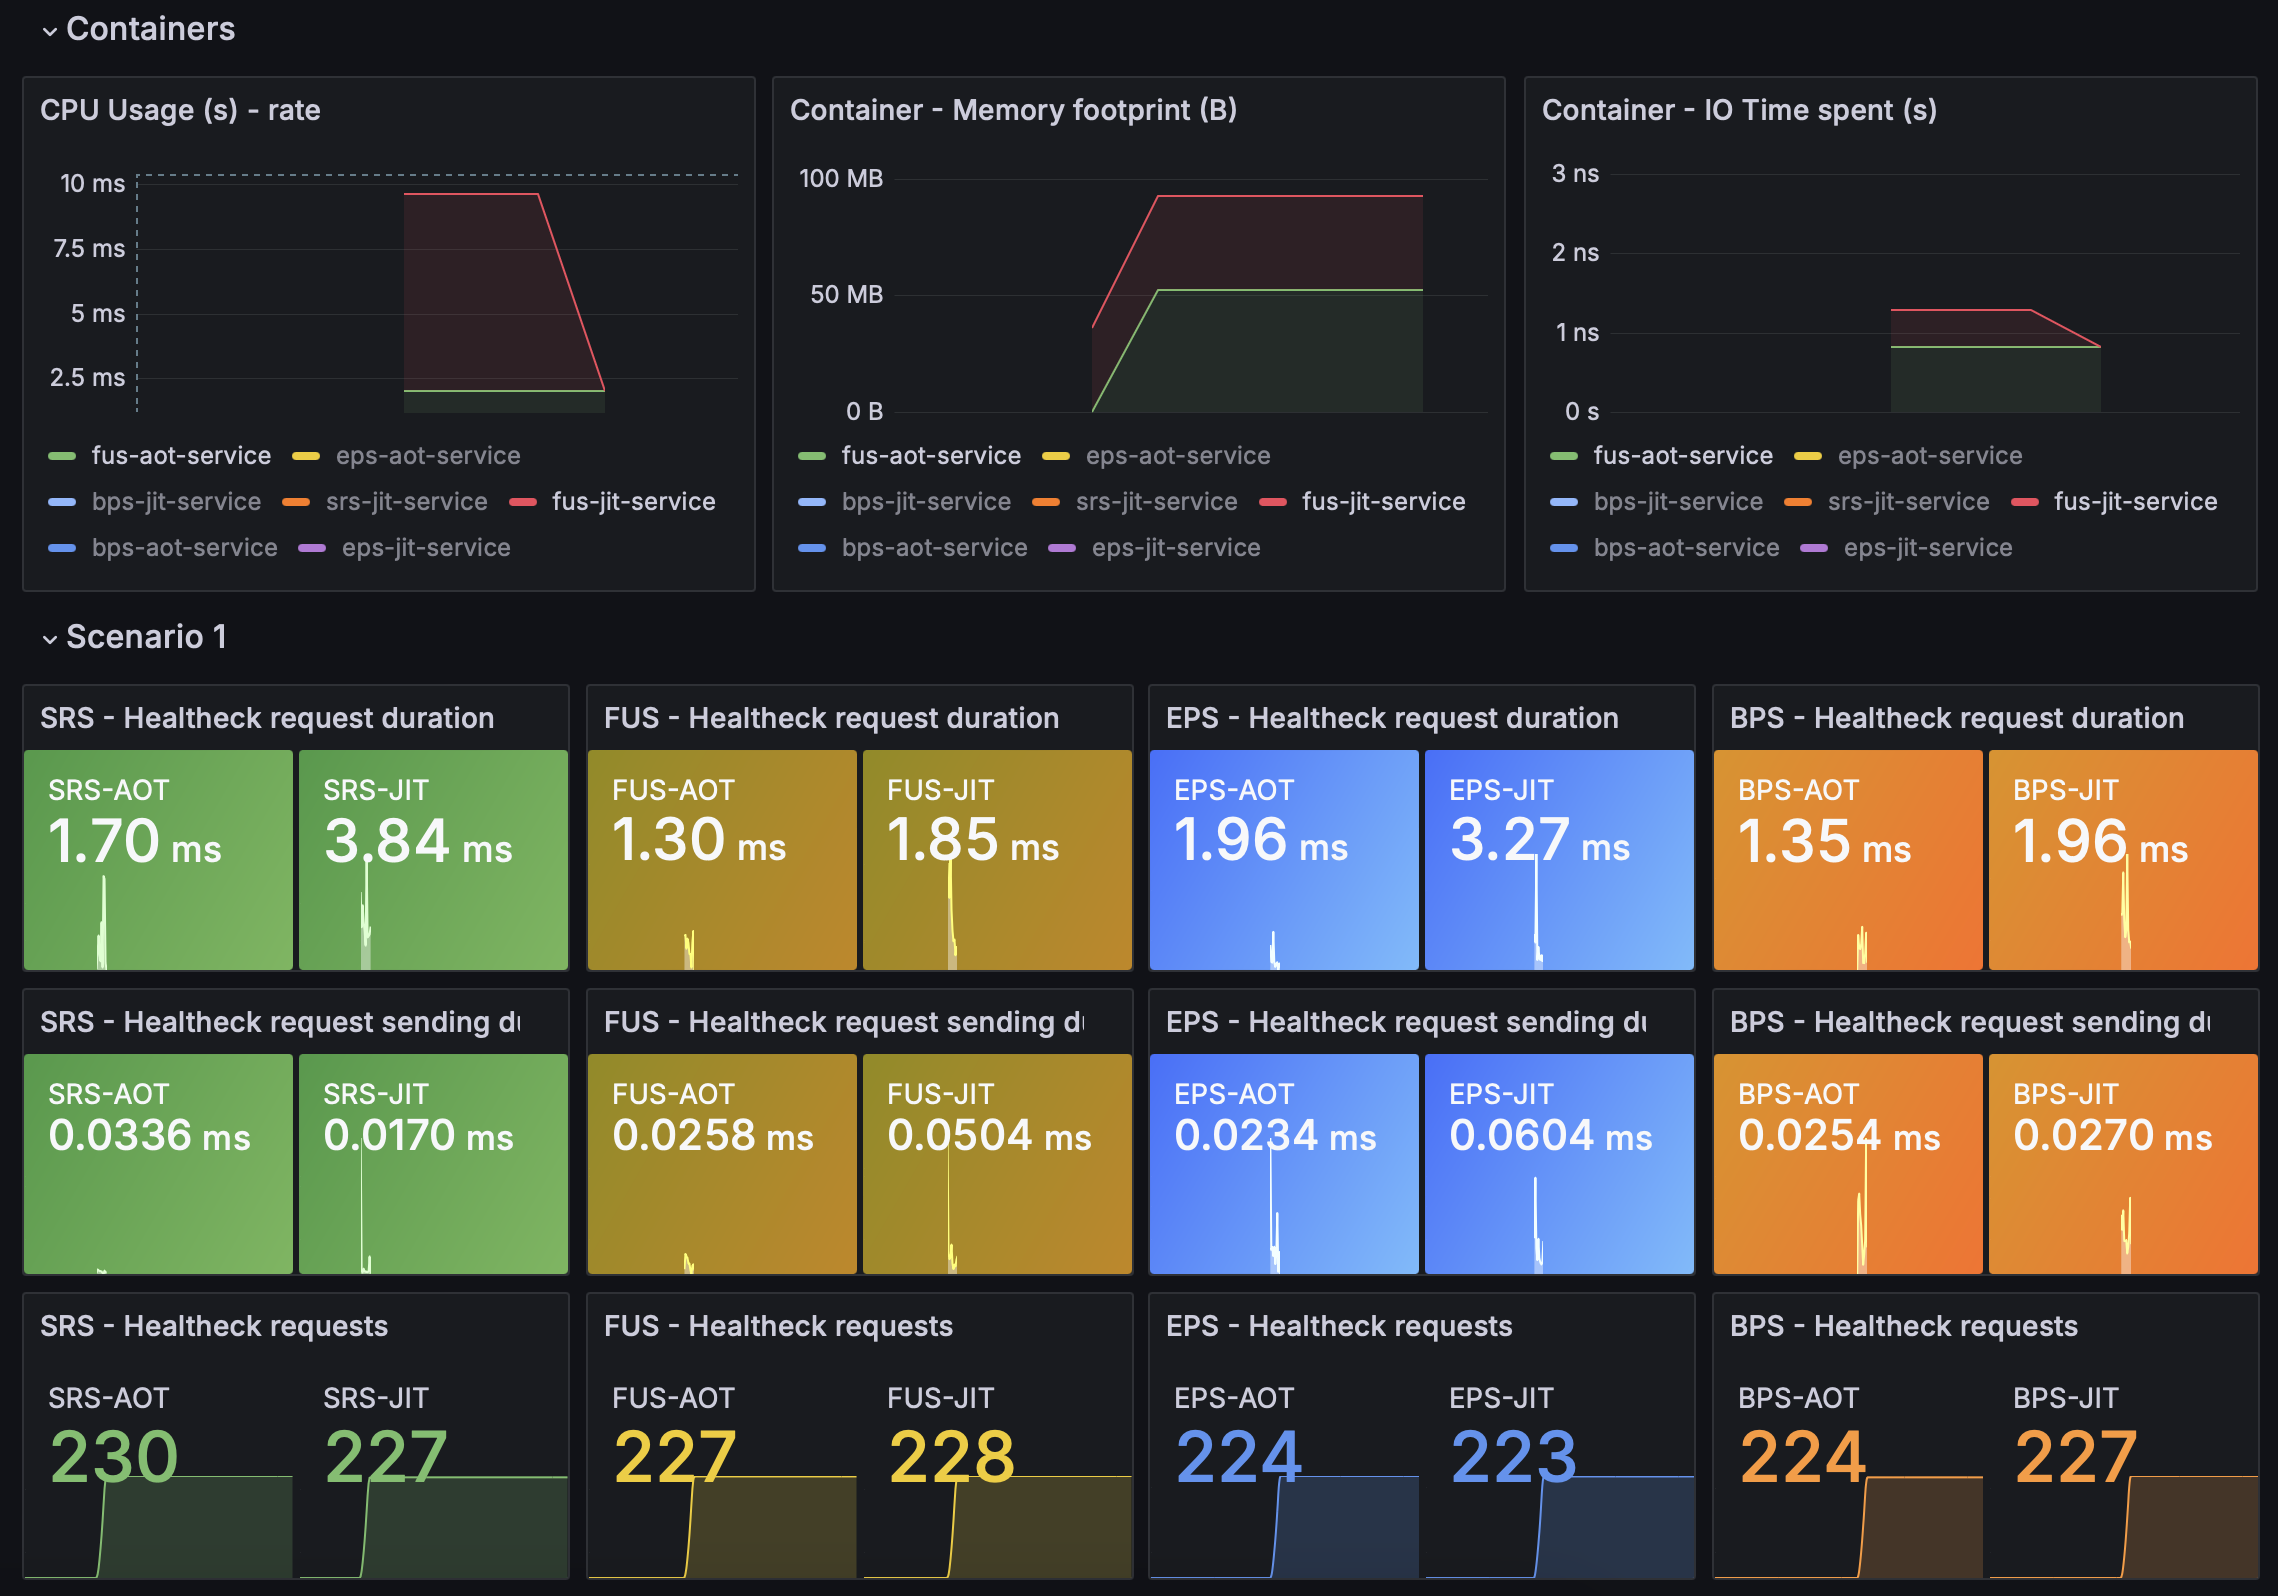
\includegraphics[width=1\textwidth]{graphics/images/scenario1-dashboard.png}
    \caption{Scénář 1 - Grafana dashboard}
    \label{fig:scenario1dashboard}
\end{figure}

% ============================================================================ %
 % Prilohy


% ============================================================================ %

\end{document}

% ============================================================================ %
